\documentclass{article}
\usepackage{ctex}
\usepackage{geometry}
\usepackage{fancyhdr}
\usepackage{zhlipsum}
\usepackage{lastpage}
\usepackage{float}
\usepackage{graphicx}
\usepackage{paralist}
\usepackage{booktabs}
\usepackage{fancybox}
\usepackage{hyperref}
\usepackage{listings}
\usepackage{xcolor}

\let\itemize\compactitem
\let\enditemize\endcompactitem
\let\enumerate\compactenum
\let\endenumerate\endcompactenum
\let\description\compactdesc
\let\enddescription\endcompactdesc

\setCJKmainfont{simsun.ttc}[BoldFont=simhei.ttf]
\geometry{a4paper,left=25mm,right=20mm,top=25mm,bottom=25mm}

\lstset{
    numbers=left,
    keywordstyle= \color{ blue!70},
    commentstyle= \color{red!50!green!50!blue!50},
    rulesepcolor= \color{ red!20!green!20!blue!20} ,
    escapeinside=``,
    numberstyle=\tt,
    numbersep=1em,
    xleftmargin=2em,
    breaklines,
    aboveskip=1em,
    framexleftmargin=3em,
    frame=shadowbox,
    basicstyle=\tt,
    language=Java
}


\title{虚拟校园系统设计说明书}

\begin{document}

\begin{titlepage}
\vspace*{\fill}

\begin{center}
    {\Huge 虚拟校园系统设计说明书}

    \vspace{10cm}
{\large
09021227~金\phantom{金}桥 \\
09021218~马晓龙 \\
09021134~王智东 \\
09021130~张博雅 \\
09021202~钟世贵 \\
09021215~曹江宁
}

    \vspace{0.5cm}
    {\large 版本:\texttt{1.0.0-draft}}

    
\vspace{0.5cm}


    {\large 日期:\today}
\end{center}

\vspace*{\fill}
\end{titlepage}
\tableofcontents
\newpage

\section{引言}
\subsection{编写目的}

本系统为东南大学计算机科学与技术专业2021级暑期学校专业技能实训课程内容。为了更清晰的描述本系统的功能以及内部运行逻辑,为代码配套编写此文档,方便后续查阅。

本文档面向系统开发、维护以及验收人员编写。

\subsection{背景}

本系统为校园系统,采用Java语言进行编写。分为服务器端与客户端:

\paragraph{服务器端}
负责运行数据库管理系统并处理来自客户端的请求并返回信息。

\paragraph{客户端}
运行在用户的计算机上,提供图形用户界面并将用户的请求发送到服务器端。同时处理服务器返回的信息并进行显示。

% \subsection{定义}
% \subsection{参考资料}


\section{程序系统的分析}

\subsection{可行性分析}

通过对学校办事大厅的调查,了解到目前学校的办事大厅整体系统结构。本系统开发的主要目的是实现校园系统的网络化,方便学校管理以及自助业务办理。

\subsection{需求分析}

项目必做部分包括以下内容:

\paragraph{用户管理}
为了实现对于用户的统一管理,我们设计了统一登录验证模块。实现对于用户的管理、登录、鉴权。

\paragraph{学生学籍管理}
为了实现学生学籍管理,我们设计了学籍管理模块,支持学生修改个人学籍信息以及教务员审核。

\paragraph{选课系统}
为了实现选课系统,我们设计了教务管理模块,支持学生选课、教师导出名单、教务员修改课程排课等功能。

\paragraph{图书馆}
参照东南大学图书馆,我们设计了图书馆管理模块,支持预约借还书、查询书籍。并支持工作人员修改书籍信息以及添加新书。

\paragraph{商店}
为了实现商店功能,我们设计了商店模块,支持用户选购商品并线上结算支付。同时支持工作人员导入货物,修改信息等。


\subsection{开发设计环境}

\subsubsection{IntelliJ IDEA}

IntelliJ IDEA是一种商业化销售的Java IDE工具软件,由JetBrains软件公司开发,提供Apache 2.0开放式授权的社区版本以及专有软件的商业版本,开发者可选择其所需来下载使用。

本系统采用IntelliJ IDEA作为开发用IDE.

\subsubsection{JDK 17}

Java 17是Java开发平台最新推出的LTS版本。Java 17 提供了数千种性能、稳定性和安全性更新,来进一步优化 Java 语言和平台,从而帮助开发人员提高工作效率。

本系统采用JDK 17作为开发平台。

\subsubsection{MySQL 8.0}

MySQL 是一个关系型数据库管理系统,由瑞典 MySQL AB 公司开发,目前属于 Oracle 公司。MySQL 是一种关联数据库管理系统,关联数据库将数据保存在不同的表中,而不是将所有数据放在一个大仓库内,这样就增加了速度并提高了灵活性。

本系统采用MySQL 8.0 作为数据库管理系统。

\subsubsection{第三方库}

\paragraph{Netty}
Netty是一个非阻塞I/O客户端-服务器框架,主要用于开发Java网络应用程序,如协议服务器和客户端。本项目采用Netty实现Socket.

\paragraph{Gson}
Gson是Google公司发布的一个开放源代码的Java库,主要用途为序列化Java对象为JSON字符串,或反序列化JSON字符串成Java对象。本项目采用Gson实现JSON格式化。

\paragraph{Slf4j与Logback}
Slf4J是一个用于日志系统的简单Facade,允许最终用户在部署其应用时使用其所希望的日志系统。Logback是一个Java日志框架,是log4j项目的继承者,性能比log4j要好。本项目采用这两者作为日志系统。

\paragraph{Hibernate}
Hibernate是一种ORM框架,全称为Object-Relative DateBase-Mapping,在Java对象与关系数据库之间建立某种映射,以实现直接存取Java对象。本项目采用Hibernate作为数据库映射。

\paragraph{Jetpack Compose}
Jetpack Compose 是Google针对Android推出的新一代声明式UI工具包,完全基于Kotlin打造,具备了跨平台的使用基础。本项目采用Jetpack Compose实现UI界面。

\section{程序系统的结构}

\begin{center}
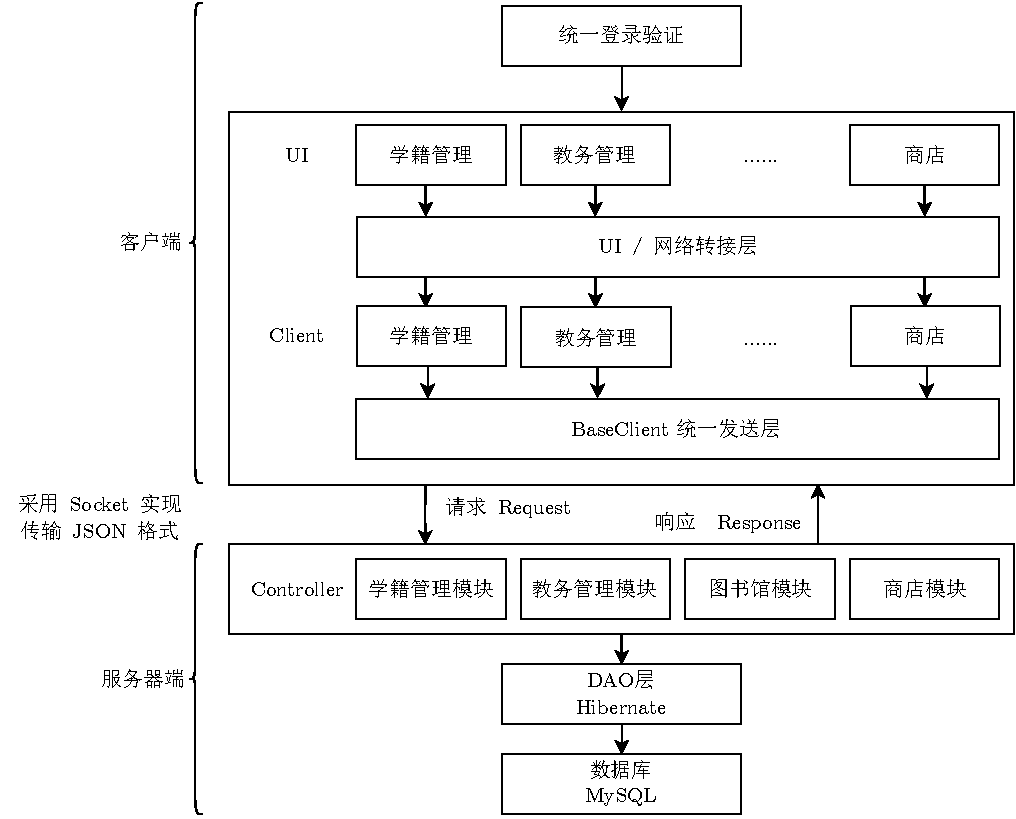
\includegraphics[width=\textwidth]{fig/full-flowchart.pdf}
\end{center}

\section{用户管理模块设计说明}
\subsection{模块背景}

统一的认证、鉴权与会话管理系统。

\subsection{需求分析}

\paragraph{登录}
实现基本的登录功能,并存储会话信息,将登录用户信息传递给其他功能模块。

\paragraph{管理}
实现用户管理功能,允许管理员便捷地管理用户,同时为用户提供部分自助功能。

\paragraph{鉴权}
配合功能模块对请求进行鉴权,根据用户身份确定其所能访问的功能,阻断非法访问请求。

\subsection{系统设计}
\subsubsection{界面设计}

\begin{center}
\shadowbox{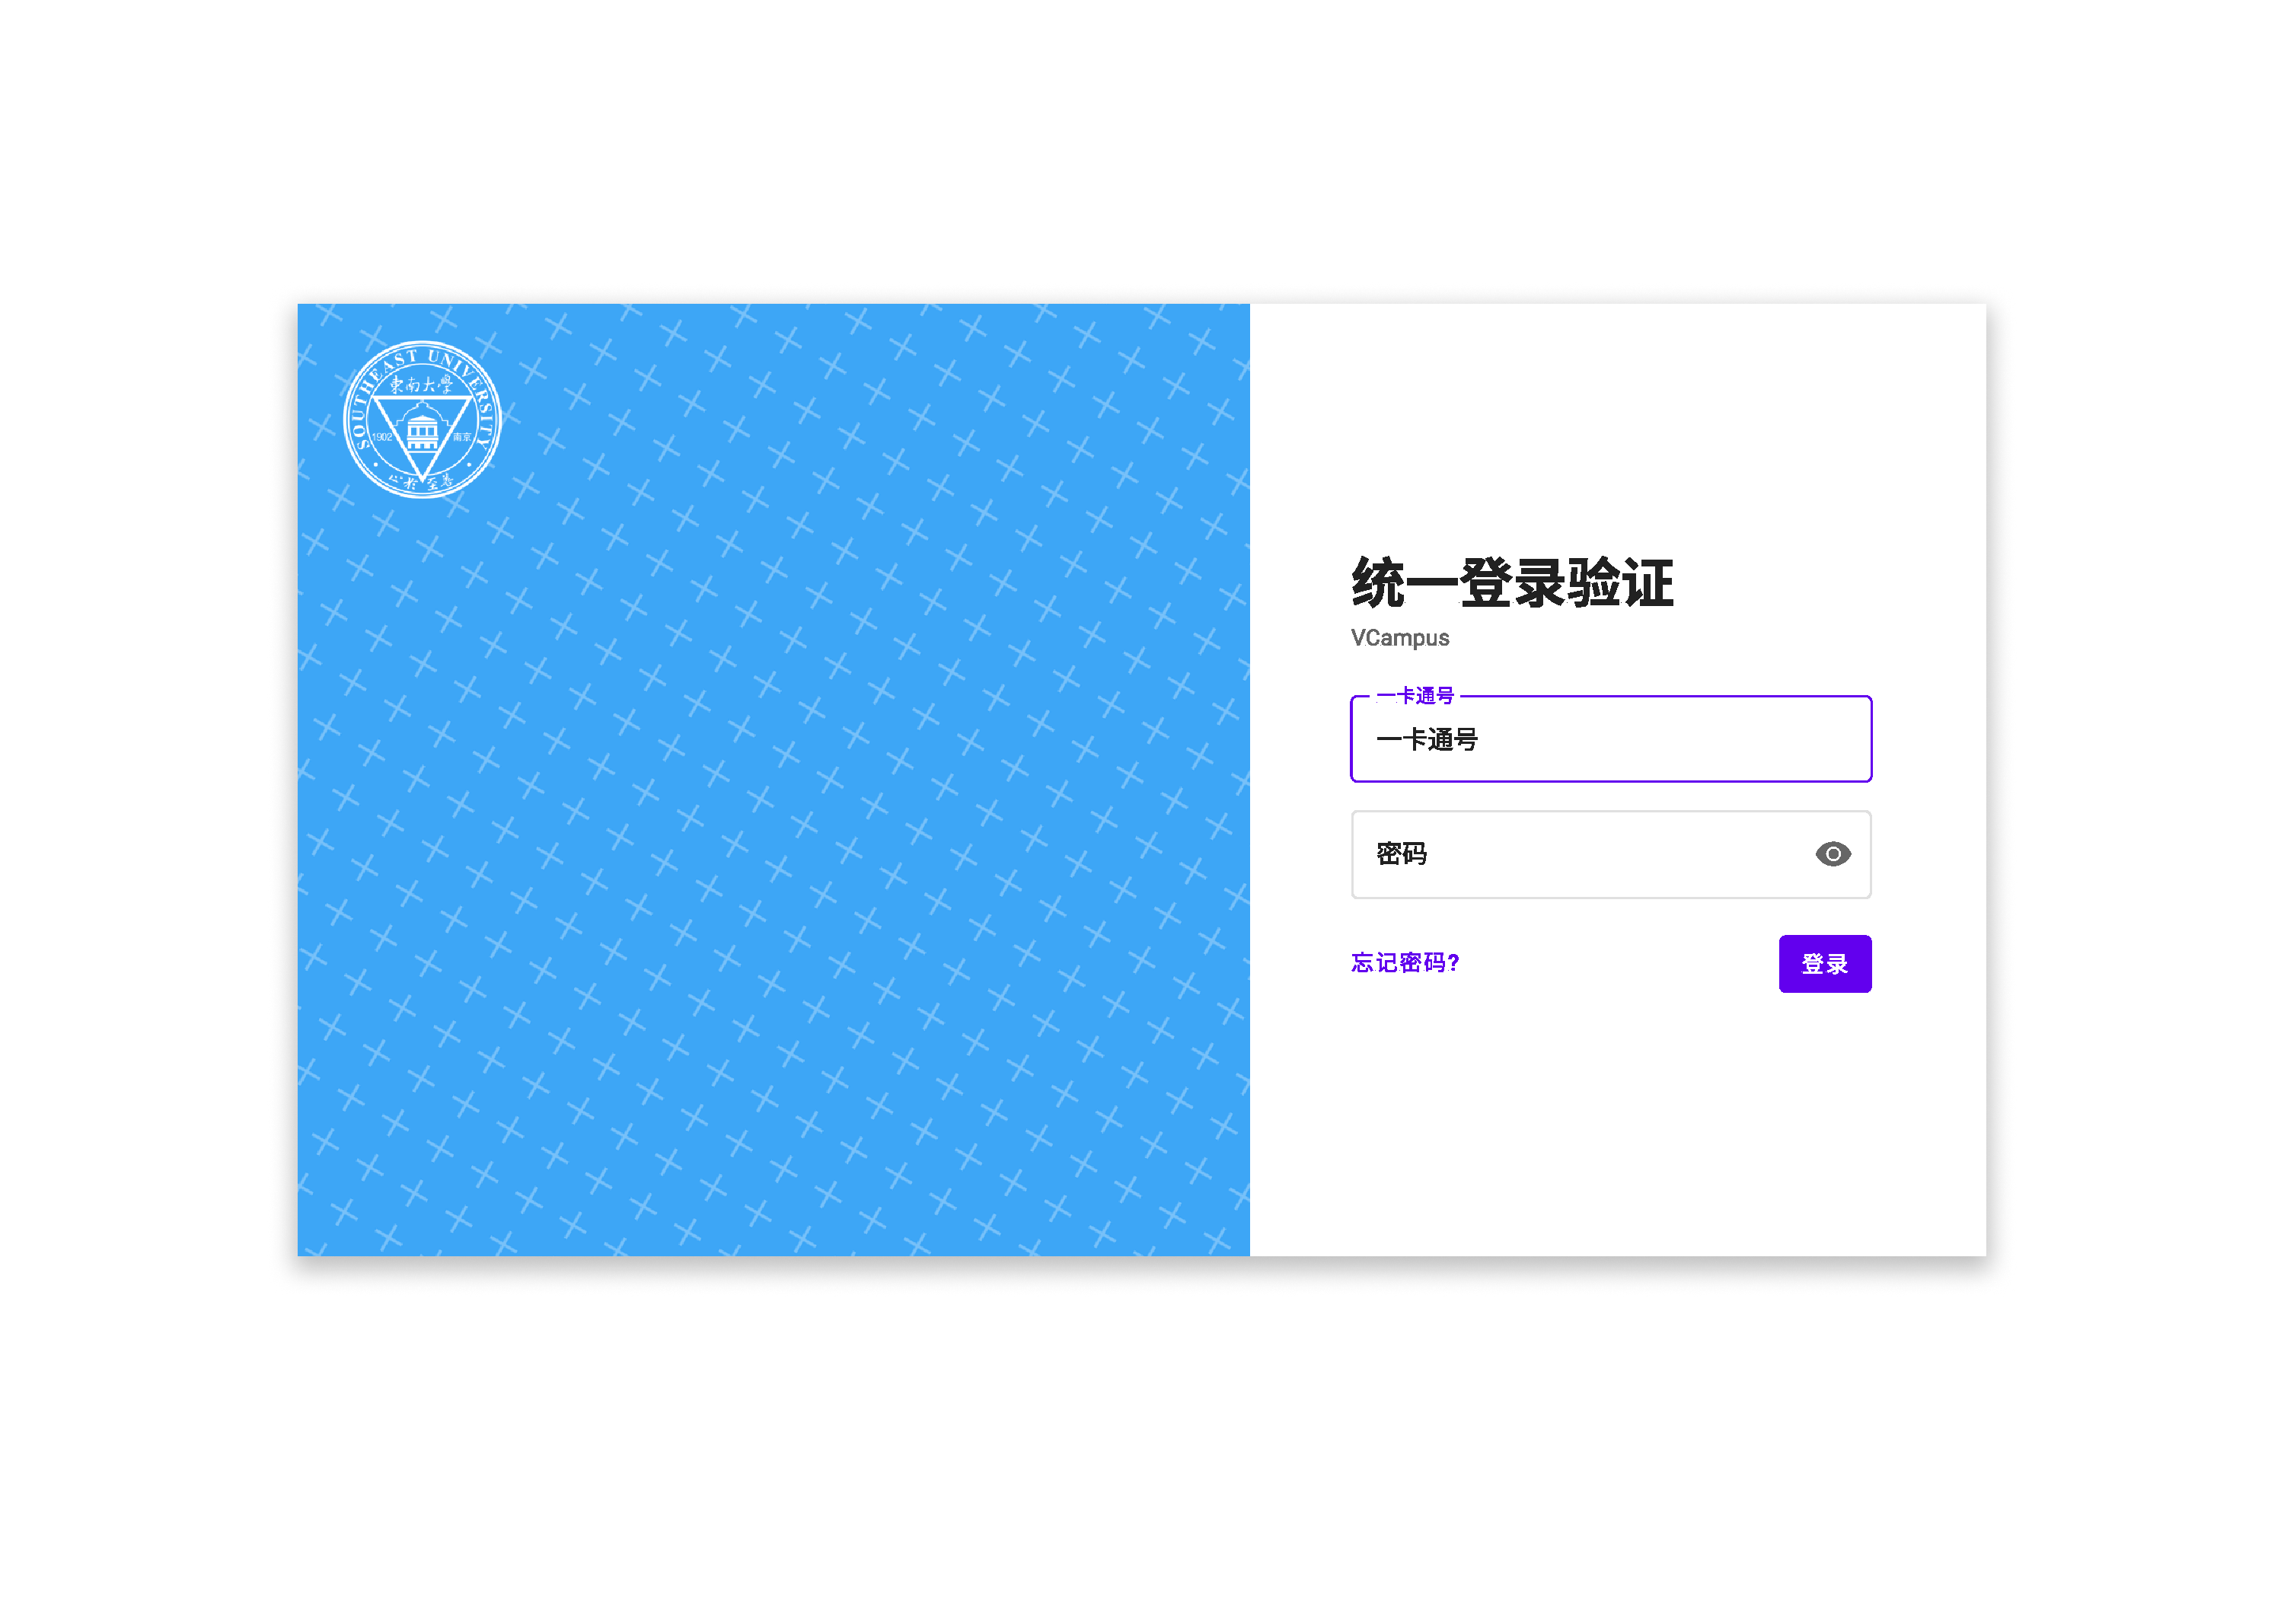
\includegraphics[width=\textwidth]{fig/uni-login-interface.pdf}}
\textbf{统一登录验证界面}
\end{center}


\subsubsection{模块流程图}

\begin{center}
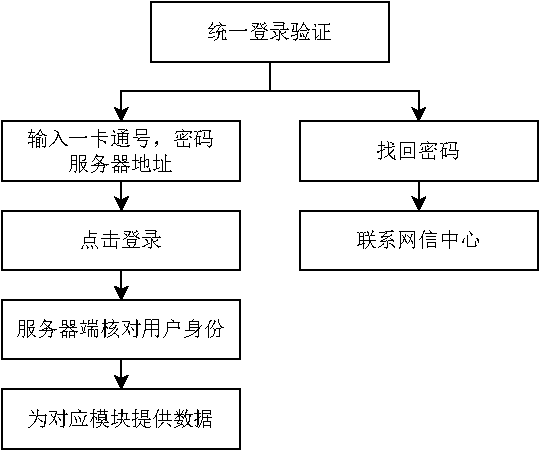
\includegraphics[width=0.5\textwidth]{fig/uni-login-flowchart.pdf}
\end{center}

\newpage

\subsubsection{类分析}

\begin{enumerate}
    \item \textbf{实体类}

    \texttt{User} 类
        \begin{table}[H]
        \centering
            \setlength{\tabcolsep}{6mm}{
                \begin{tabular}{ccccc}
                \hline
                序号    & 名称    & 类型    & 约束    & 备注\\
                \hline
                1 & \texttt{cardNumber} & \texttt{Integer}   & 9位数字 & 一卡通号\\
                2 & \texttt{password} & \texttt{String} &  & 处理后的密码\\
                3 & \texttt{name}  & \texttt{Integer} &  & 姓名\\
                4 & \texttt{gender}  & \texttt{enum} &  & 性别\\
                5 & \texttt{phone}   & \texttt{String} &  & 手机号\\
                6 &\texttt{email}  & \texttt{String} &  & 邮箱\\
                7 &\texttt{role}  & \texttt{String} &  & 权限角色\\
                \hline
        \end{tabular}}
        \end{table}
        
    \item \textbf{服务类}

    客户端:\texttt{AuthClient}
    \begin{table}[H]
        \centering
            \setlength{\tabcolsep}{6mm}{
                \begin{tabular}{cccc}
                \hline
                序号    & 名称    & 方法    & 备注\\
                \hline
                1 & 登录 & \texttt{login} & 使用密码登录\\
                2 & 登出 & \texttt{logout} & 退出登录\\
                3 & 重置密码 & \texttt{resetPassword} & 验证后重置密码\\
                \hline
        \end{tabular}}
        \end{table}
    
    服务器端:\texttt{AuthController}
    \begin{table}[H]
        \centering
            \setlength{\tabcolsep}{6mm}{
                \begin{tabular}{cccc}
                \hline
                序号    & 名称    & 方法    & 备注\\
                \hline
                1 & 登录 & \texttt{login} & 使用密码登录\\
                2 & 登出 & \texttt{logout} & 退出登录\\
                3 & 重置密码 & \texttt{resetPassword} & 验证后重置密码\\
                \hline
        \end{tabular}}
        \end{table}

\end{enumerate}

\section{学籍管理模块设计说明}
\subsection{模块背景}
  用于管理学生的学籍相关信息。
\subsection{需求分析}

\paragraph{学生端}
学生可以通过该模块查看、更新、填写自己的学籍信息相关内容,比如一卡通号、学号、专业编号及名称、学院编号及名称、学籍状态、入学时间等。

\paragraph{教务端}
教务管理人员可以通过该模块审核、管理、修改相关学生的学籍信息。在学生首次填写及后续更改自己的学籍信息后,教务负责审核该信息是否合法、正确。并且可以根据学院相关规章、要求对学生的信息进行后台更改。
\begin{center}
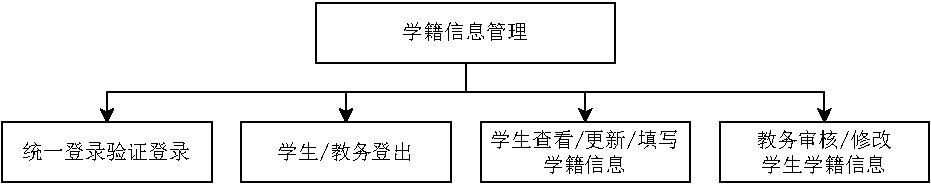
\includegraphics[width=0.8\textwidth]{fig/student-status-demand-flowchart.pdf}
\end{center}
\subsection{系统设计}
\subsubsection{界面设计}

\begin{center}
\shadowbox{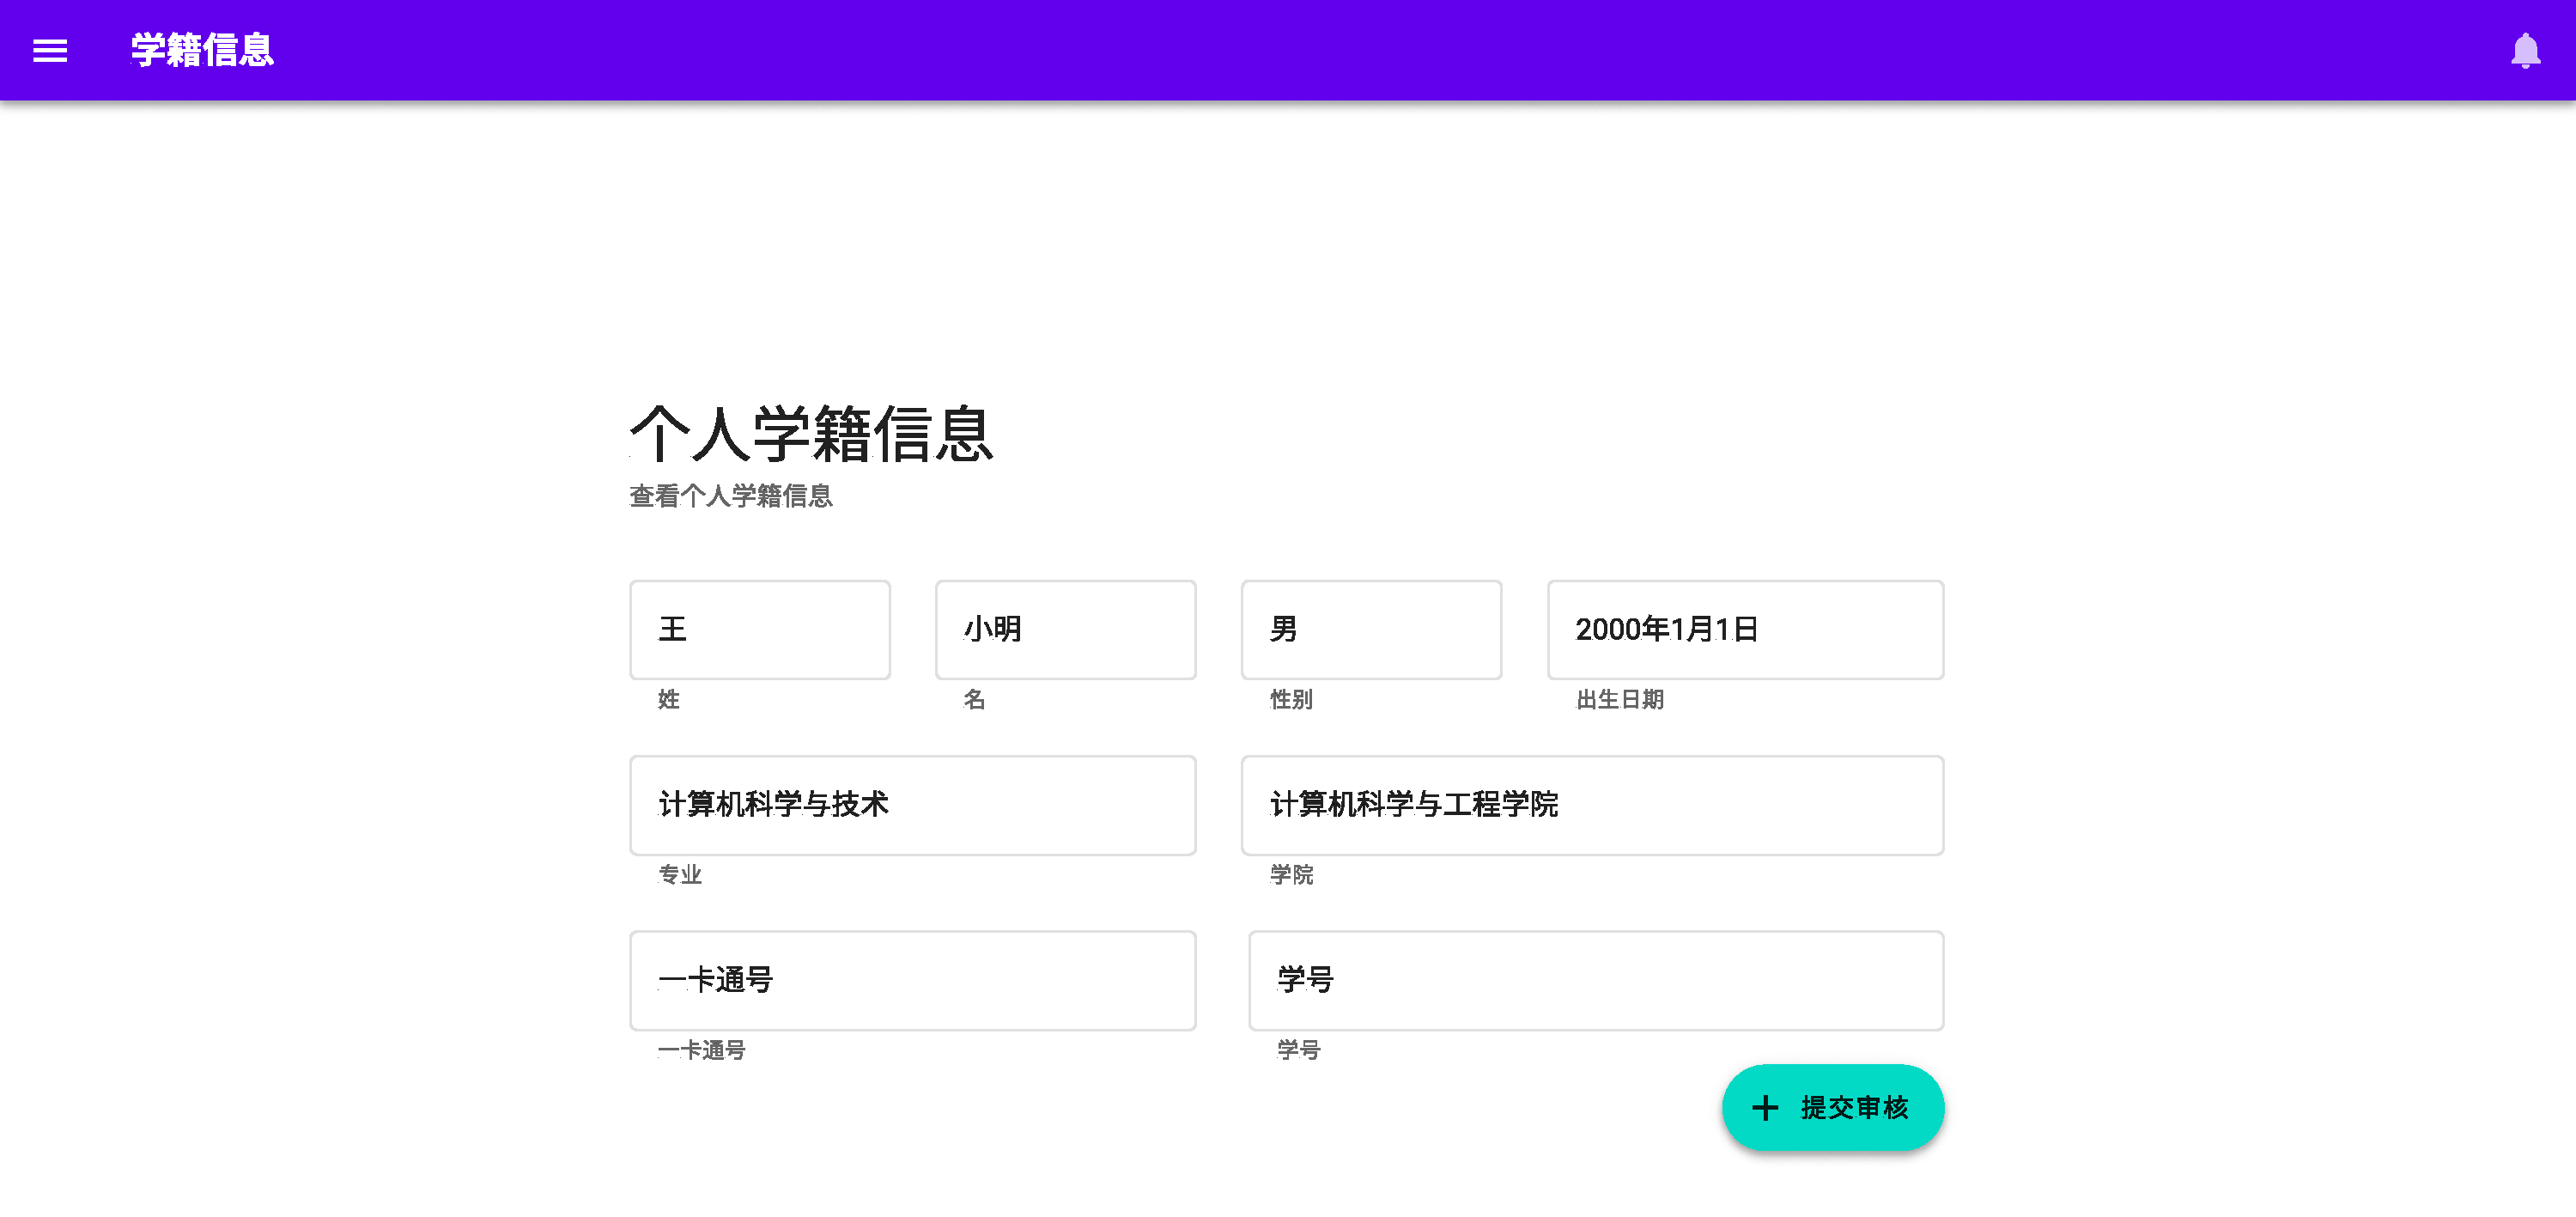
\includegraphics[width=\textwidth]{fig/profile-interface.pdf}}
\textbf{学生端操作界面}
\end{center}

\begin{center}
\shadowbox{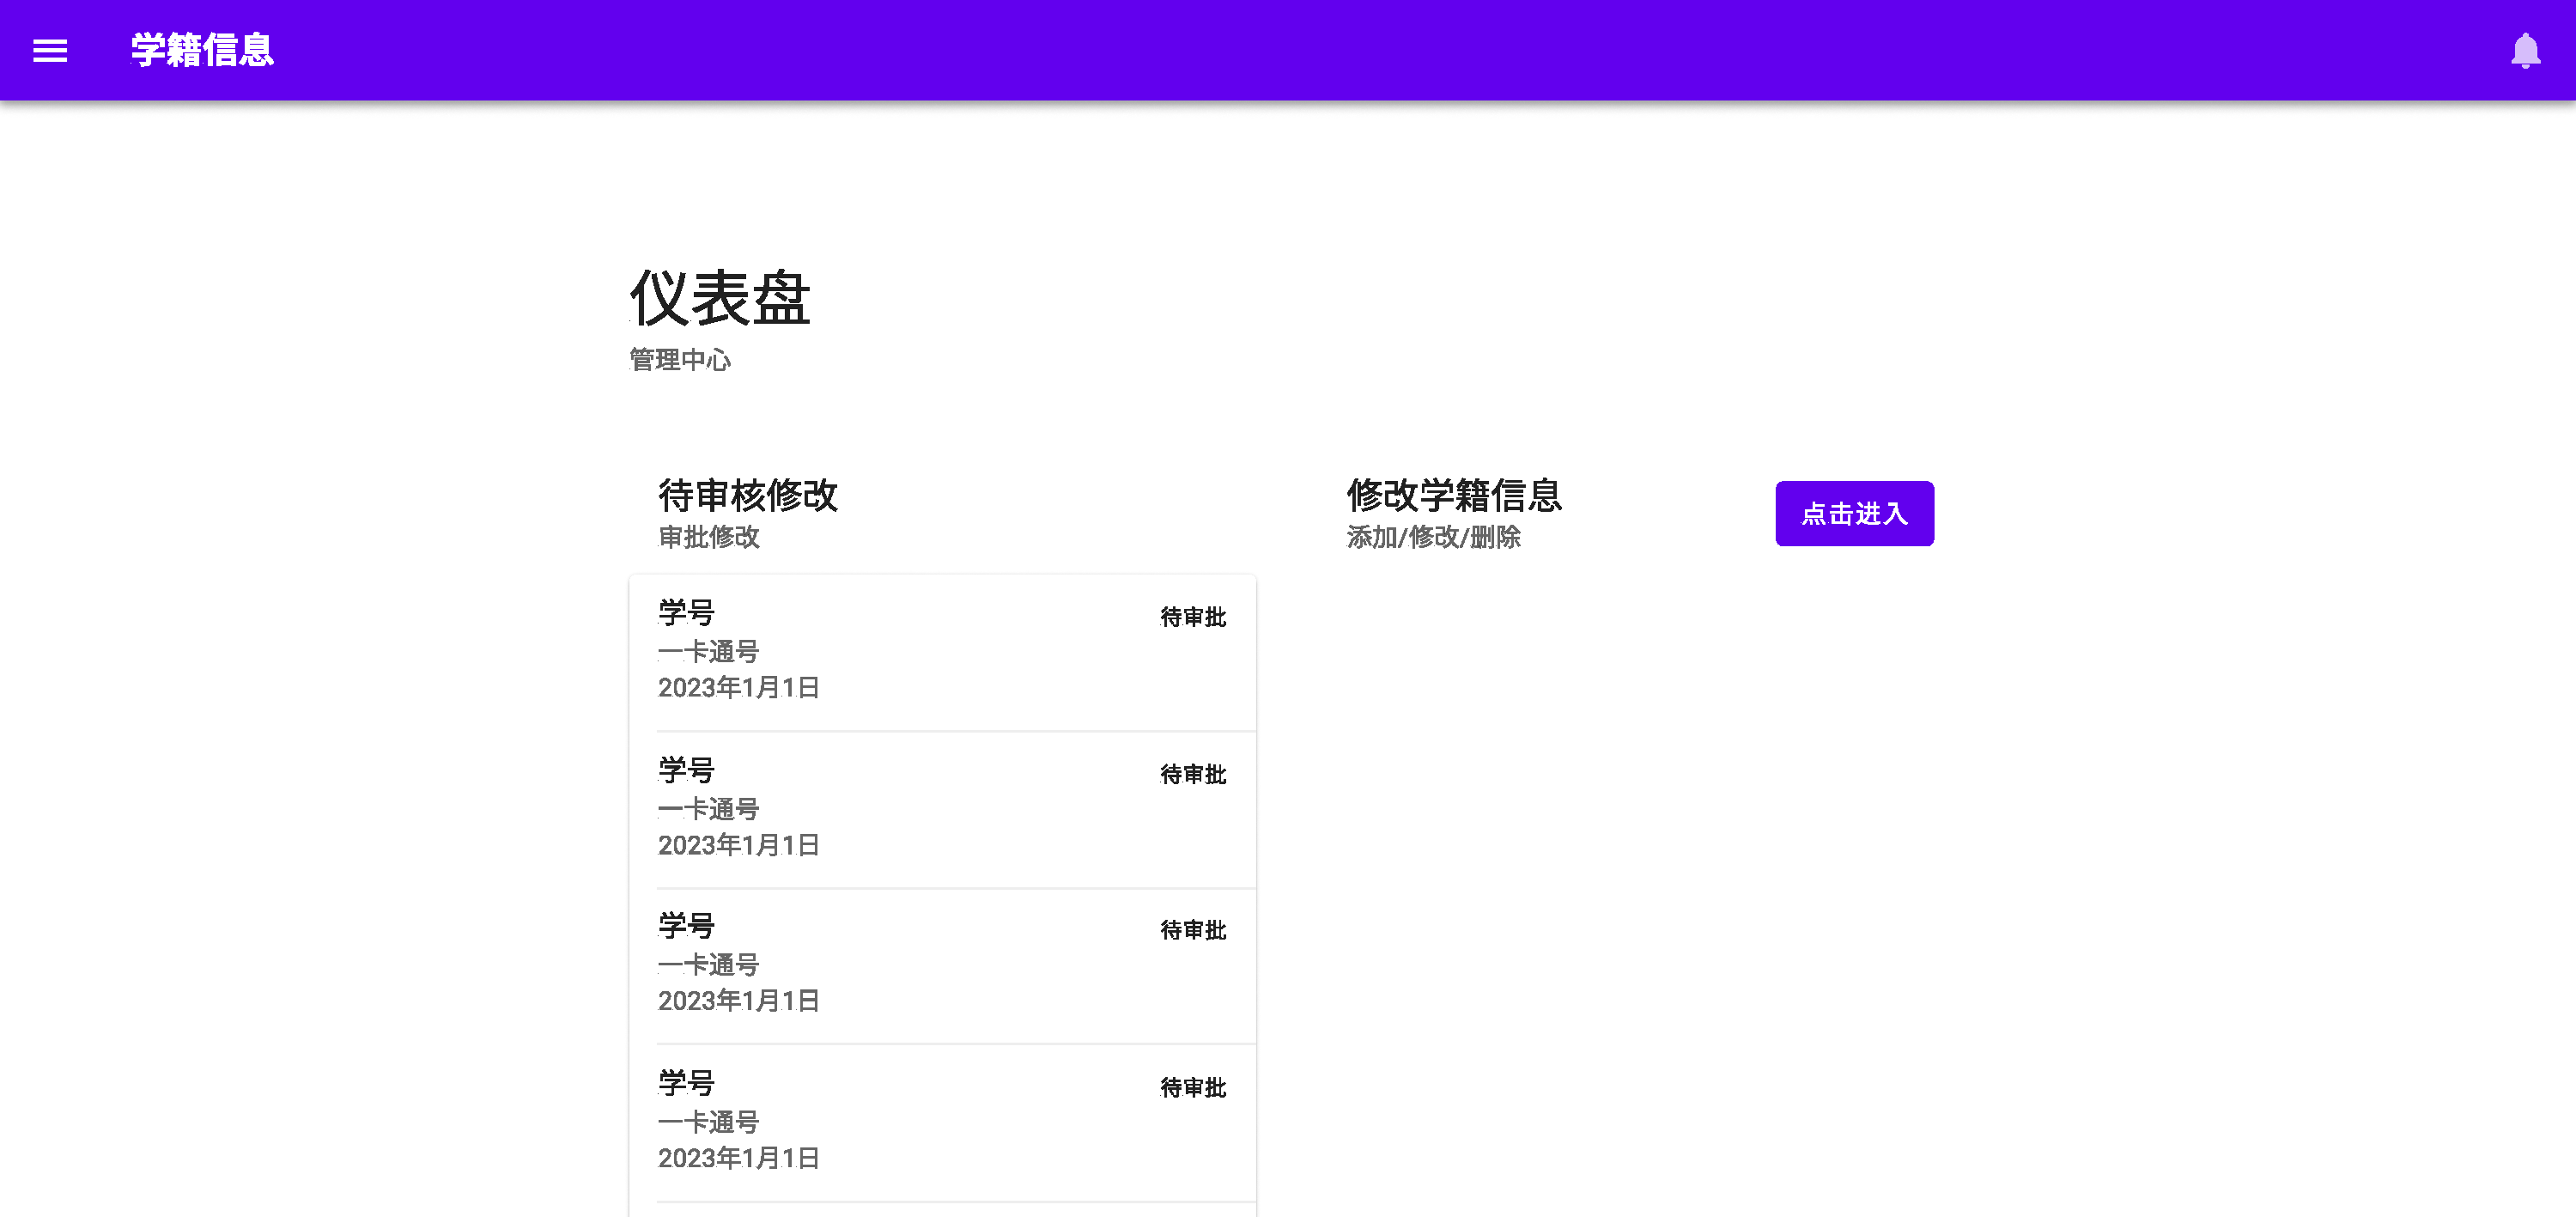
\includegraphics[width=\textwidth]{fig/profile-dashboard-interface.pdf}}
\textbf{教务端操作界面}
\end{center}

\subsubsection{模块流程图}
\begin{center}
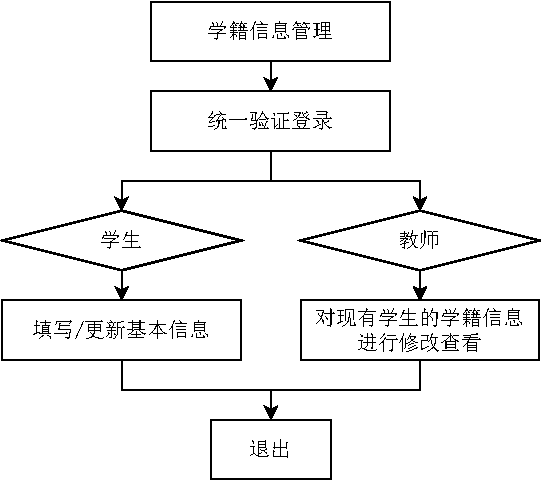
\includegraphics[width=0.5\textwidth]{fig/student-status-flowchart.pdf}
\end{center}
\subsubsection{类分析}
\begin{enumerate}
    \item 
    实体类:

    学生类:\texttt{Student}
        \begin{table}[H]
        \centering
            \setlength{\tabcolsep}{6mm}{
                \begin{tabular}{ccccc}
                \hline
                序号&名称    & 类型 & 约束  & 备注\\
                \hline
                1&\texttt{cardNumber} & \texttt{Integer} & 9位数字 & 一卡通号\\
                2&\texttt{studentNumber} & \texttt{String} & 8位数字 & 学号\\
                3&\texttt{major}  & \texttt{Integer} & & 专业编号用于索引\\
                4&\texttt{school} & \texttt{Integer} & & 学院编号用于索引\\
                5&\texttt{status}  & \texttt{enum} &  & 学籍状态(在读/离职等)\\
                6&\texttt{enrollment} &\texttt{calendar} & &入学日期(年/月/日)\\
                7&\texttt{birthPlace}  &\texttt{String}  &  &籍贯\\
                8&\texttt{politicalStat}    &\texttt{enum}  &    &政治面貌\\
                \hline
        \end{tabular}}
        \end{table}


    专业类(存放专业编号及名称):\texttt{Major}

\begin{table}[H]
  \centering
  \setlength{\tabcolsep}{10mm}{
    \begin{tabular}{ccccc}
    \hline
    序号&名称    & 类型 & 约束  & 备注\\
    \hline
    1&\texttt{majorNum} & \texttt{Integer} &  & 专业编号\\
    2&\texttt{majorName} & \texttt{String} & & 专业名称\\
    \hline
    \end{tabular}}
\end{table}


学院类(存放学院编号及名称):\texttt{School}

\begin{table}[H]
  \centering
  \setlength{\tabcolsep}{10mm}{
    \begin{tabular}{ccccc}
    \hline
    序号&名称    & 类型 & 约束  & 备注\\
    \hline
    1&\texttt{schoolNum} & \texttt{Integer} &  & 学院编号\\
    2&\texttt{schoolName} & \texttt{String} & & 学院名称\\
    \hline
    \end{tabular}}
\end{table}
    \newpage
    \item \textbf{服务类}

    客户端:\texttt{StudentStatusClient}
        \begin{table}[H]
        \centering
            \setlength{\tabcolsep}{10mm}{
                \begin{tabular}{cccc}
                \hline
                序号 & 名称    & 方法    & 备注\\
                \hline
                1 & 发送  &\texttt{stuInfoFetch}   &发request\\
                2 & 添加  &\texttt{requestInfo}    &发送个人信息\\
                3 & 更新  &\texttt{updataInfo}     &更新个人信息\\
                4 & 修改  &\texttt{modifyInfo}     &修改个人信息\\
                5 & 保存  &\texttt{saveInfo}       &保存个人信息\\
                \hline
        \end{tabular}}
    \end{table}

    服务器端:\texttt{StudentStatusController}
    \begin{table}[H]
        \centering
            \setlength{\tabcolsep}{10mm}{
                \begin{tabular}{cccc}
                \hline
                序号 & 名称    & 方法    & 备注\\
                \hline
                1 & 添加个人信息    & \texttt{addInfoHandle}  &添加个人信息\\
                2 & 删除个人信息    & \texttt{deleteInfoHandle} &删除个人信息\\
                3 & 更新个人信息    & \texttt{updateInfoHandle}  &更新个人信息\\
                4 & 暂存个人信息    & \texttt{saveInfoHandle}     &暂存个人信息\\
                5 & 修改个人信息    & \texttt{modifyInfoHandle}    &修改个人信息\\
                  \hline
        \end{tabular}}
    \end{table}



\end{enumerate}

\section{教务管理模块设计说明}
\subsection{模块背景}
  用于管理教务的相关信息。
\subsection{需求分析}

\paragraph{课程管理功能} 包括课程创建与编辑、课程计划以及课程信息发布功能。

·课程创建与编辑:教务管理员能够创建新的课程,指定课程名称、课程编号、学分、授课老师、开设学院等信息,并可以编辑课程信息。

·课程计划:管理员可以制定每学期的课程计划,安排各门课程的时间、地点和教师,确保课程表的合理性和平衡性。

·课程信息发布:将课程信息、教师信息、教室信息等发布给学生和教师,以便学生能够及时了解课程安排。

\paragraph{排课功能}
教务员能够根据不同专业的学生人数及课程相关信息,排出合理课程表,避免时间冲突。

\paragraph{成绩管理功能}
教师能够录入学生的考试成绩和平时成绩,并提供学生查询自己的成绩。

\subsection{系统设计}
\subsubsection{界面设计}

\begin{center}
\shadowbox{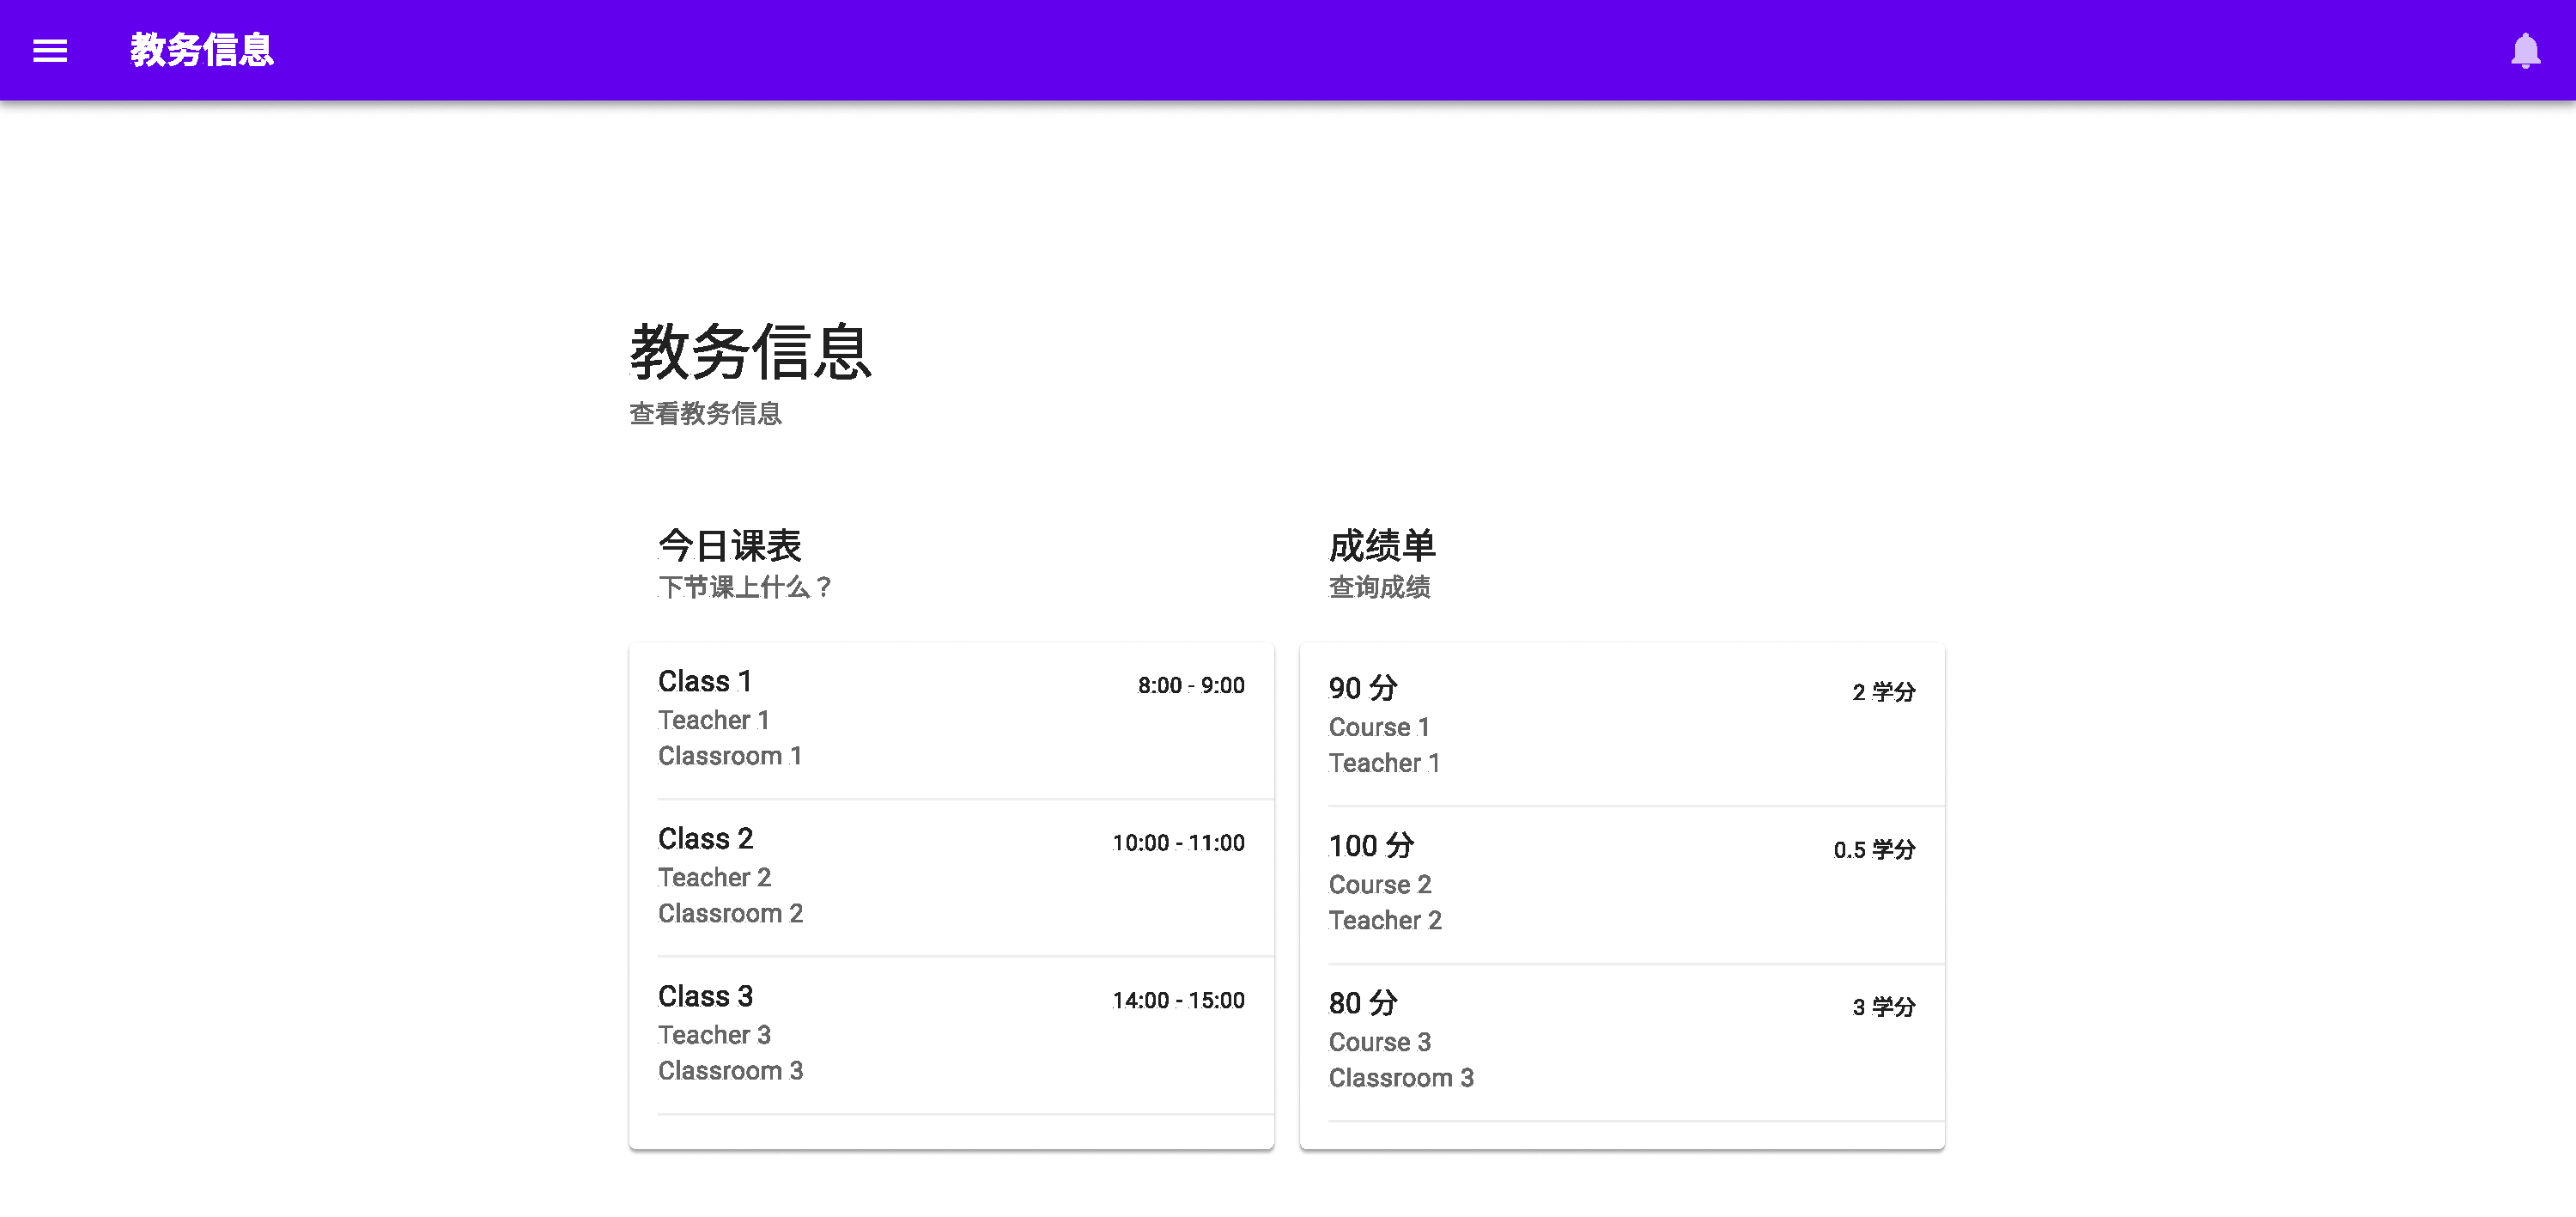
\includegraphics[width=\textwidth]{fig/affair-interface.pdf}}
\textbf{学生端操作界面}
\end{center}

\begin{center}
\shadowbox{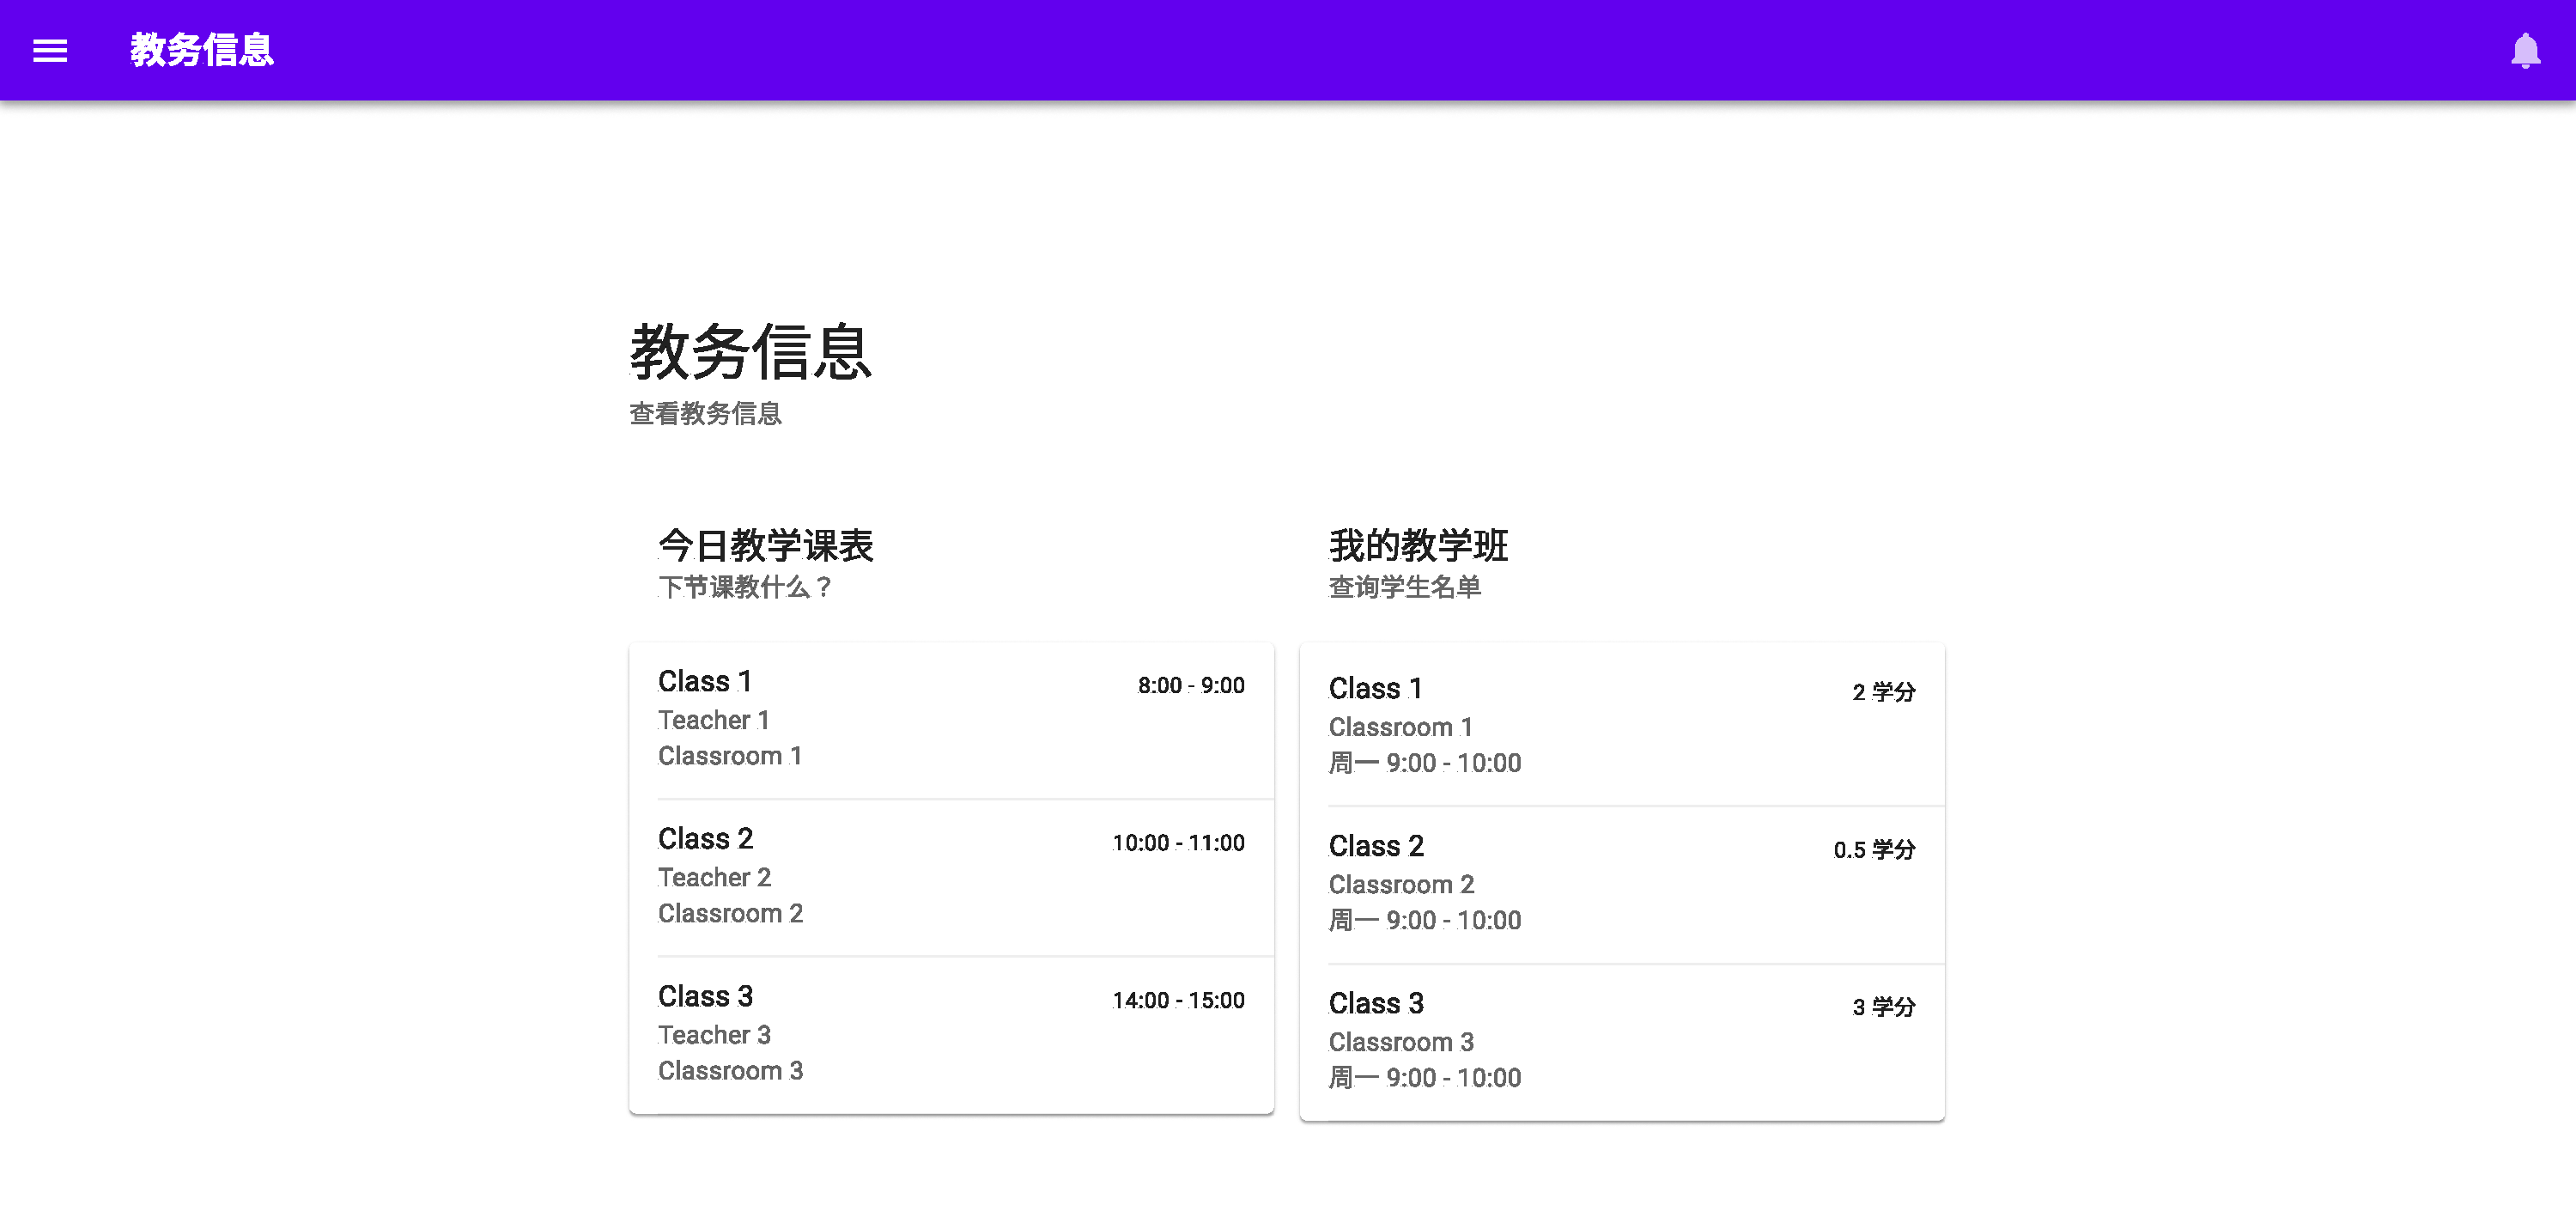
\includegraphics[width=\textwidth]{fig/affair-teacher-interface.pdf}}
\textbf{教师端操作界面}
\end{center}

\begin{center}
\shadowbox{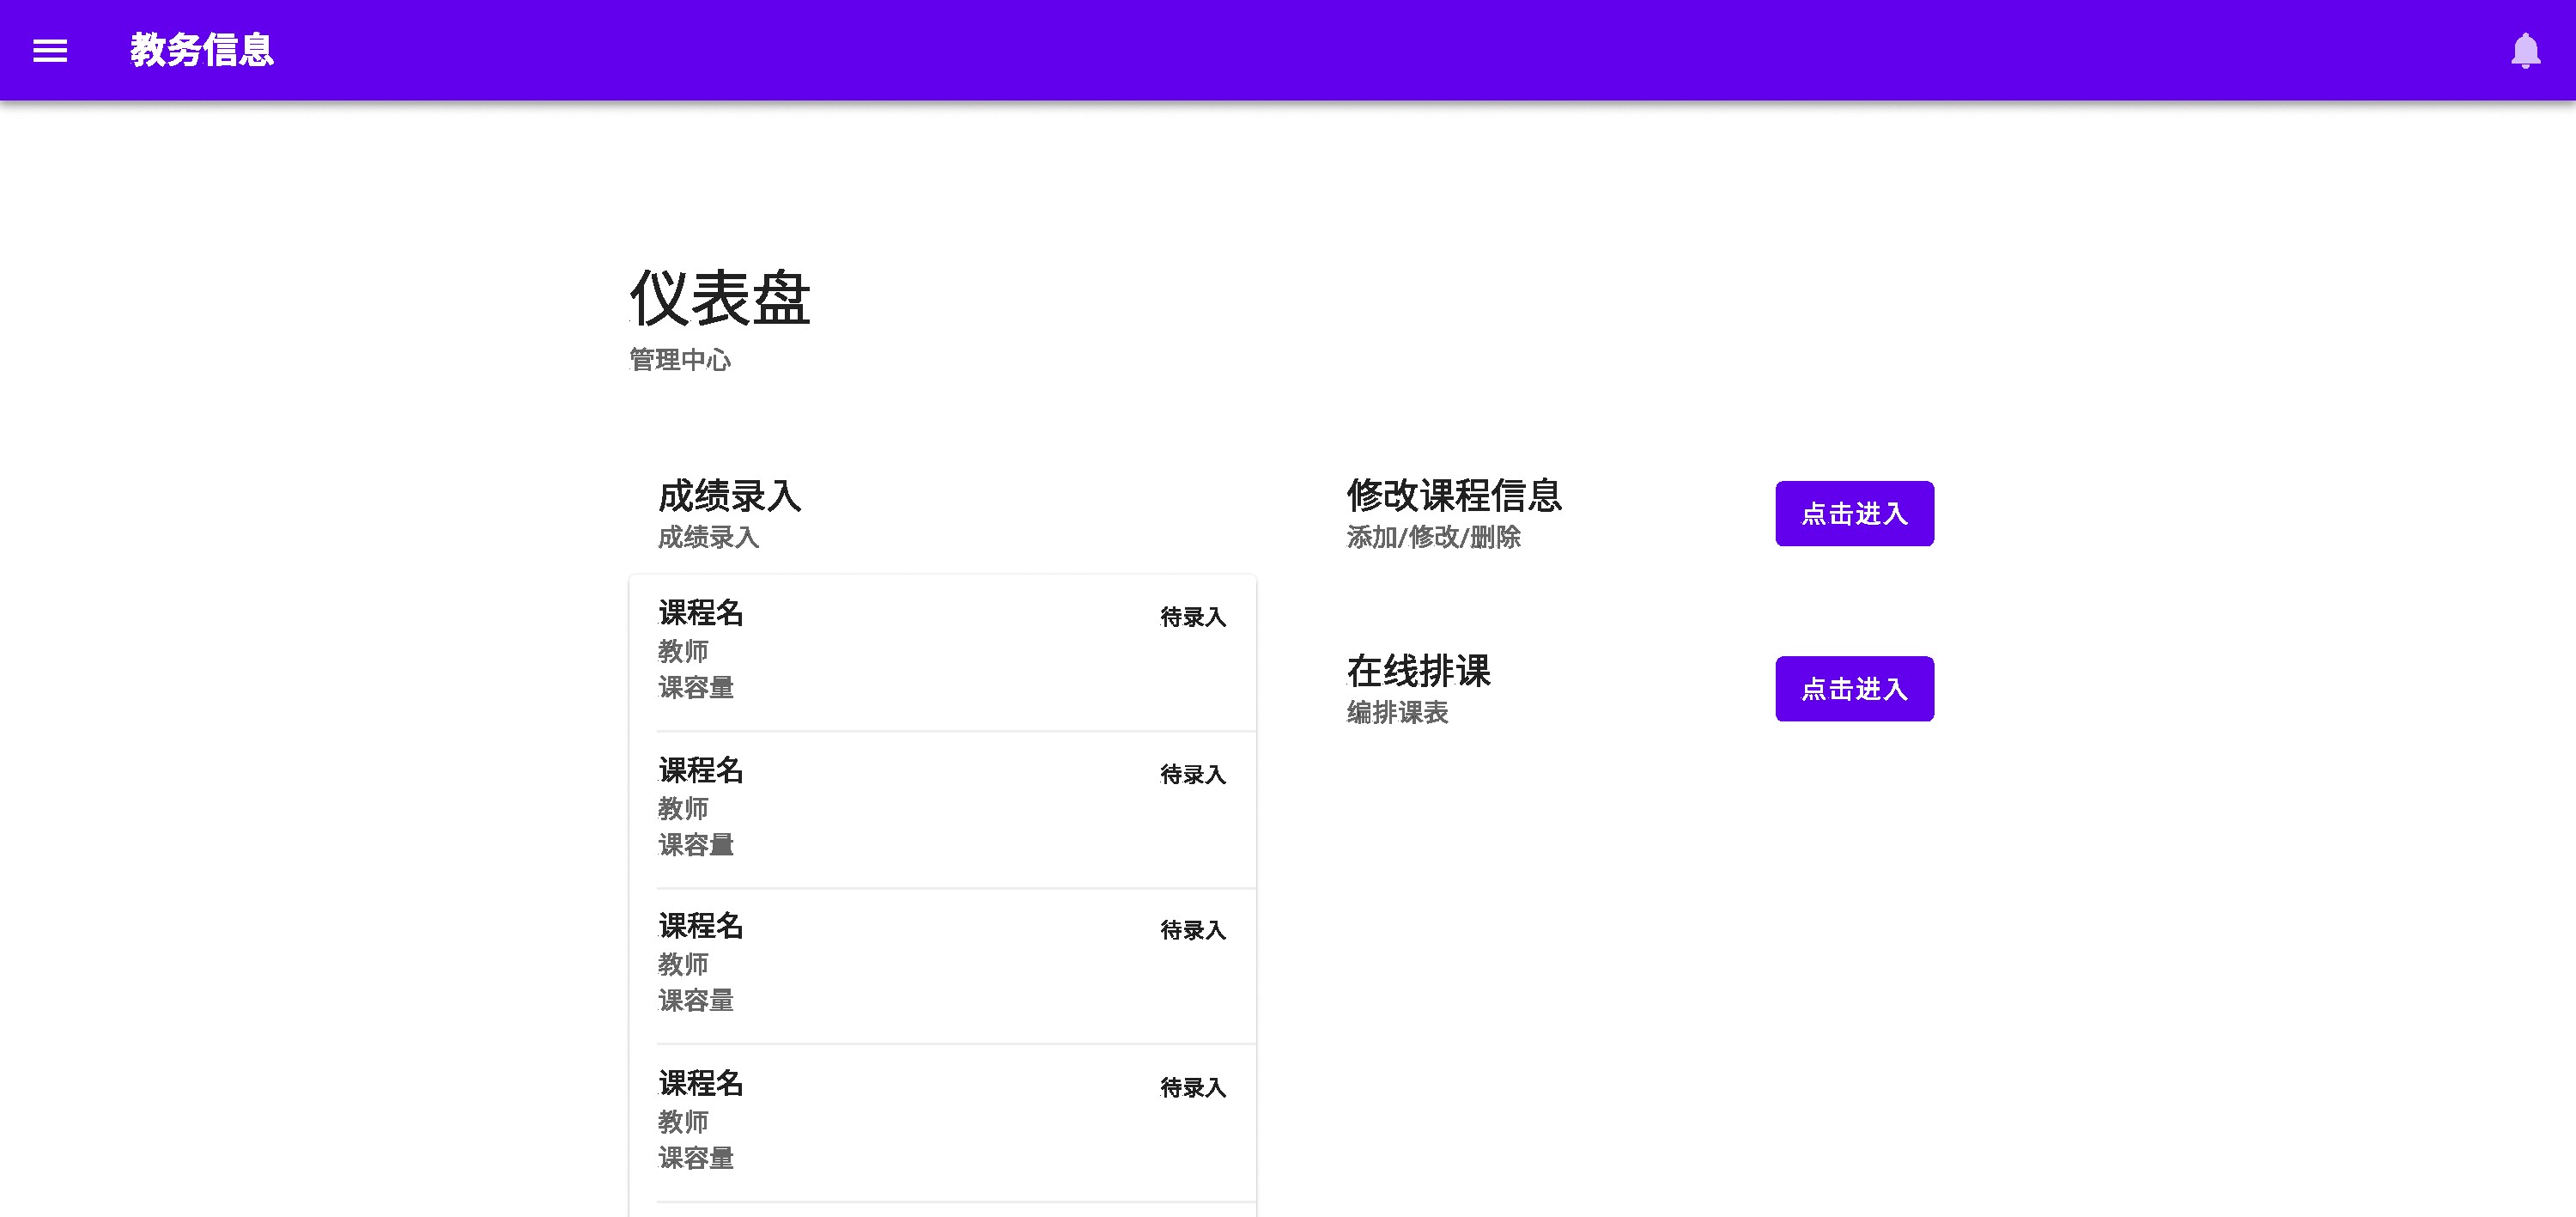
\includegraphics[width=\textwidth]{fig/affair-dashboard-interface.pdf}}
\textbf{教务端操作界面}
\end{center}

\subsubsection{模块流程图}

\begin{center}
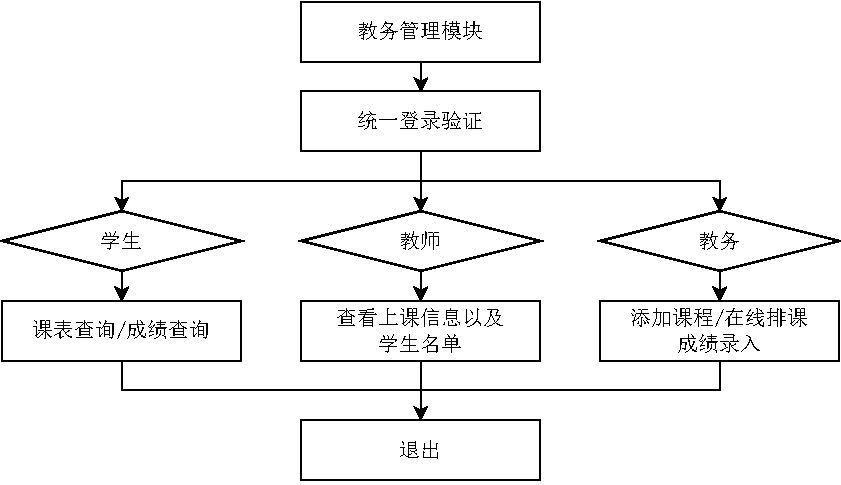
\includegraphics[width=0.7\textwidth]{fig/affair-flowchart.pdf}
\end{center}

\newpage

\subsubsection{类分析}

\begin{enumerate}
\item \textbf{实体类}

学生类:\texttt{Student}
\begin{table}[H]
   \centering
    \begin{tabular}{ccccc}
    \hline
    序号&名称    & 类型    & 约束    & 备注 \\
    \hline
    1&\texttt{cardNumber} & \texttt{Integer}   & 9位数字  & 学生一卡通号 \\
    2&\texttt{studentNumber} & \texttt{Integer}   & 8位数字  & 学号 \\
    3&\texttt{major} & \texttt{Integer}   &  & 专业编号 \\
    4&\texttt{school} & \texttt{Integer}   &  & 学院编号 \\
    5&\texttt{status} & \texttt{enum}   &  & 学籍状态 \\
    6&\texttt{enrollment} & \texttt{calendar}   &  & 入学日期 \\
    7&\texttt{birthPlace} & \texttt{String}   &  & 籍贯 \\
    8&\texttt{poliStat} & \texttt{enum}   &  & 政治面貌 \\
    \hline
    \end{tabular}%
\end{table}

开设课程的基本信息类:\texttt{Course}
\begin{table}[H]
  \centering
    \begin{tabular}{ccccc}
    \hline
    序号&名称    & 类型    & 约束    & 备注 \\
    \hline
    1&\texttt{uui}d  & \texttt{UUID}  &       & 唯一标识符,用作主键 \\
    2&\texttt{courseId} & \texttt{Integer}   &  & 课程编号 \\
    3&\texttt{courseName} & \texttt{String} &       & 课程名 \\
    4&\texttt{school} & \texttt{String} &       & 开设学院 \\
    5&\texttt{credit} & \texttt{float} &       & 学分 \\
    \hline
    \end{tabular}%
\end{table}%

教学班的基本信息类:\texttt{Class}

\begin{table}[H]
  \centering
    \begin{tabular}{ccccc}
    \hline
    序号&名称    & 类型    & 约束    & 备注 \\
    \hline
    1&\texttt{uuid}  & \texttt{UUID}  &       & 唯一标识符,用作主键 \\
    2&\texttt{courseId} & \texttt{Integer}   &       & 课程编号 \\
    3&\texttt{courseName} & \texttt{String} &       & 课程名 \\
    4&\texttt{teacherId} & \texttt{Integer}   &       & 教师编号 \\
    5&\texttt{schedule} & \texttt{String} &       & 上课信息 \\
    6&\texttt{place} & \texttt{string} &  & 上课地点 \\
    7&\texttt{capacity} & \texttt{String} &       & 上课信息 \\
    \hline
    \end{tabular}%
\end{table}%

学生所选课程的基本信息类:\texttt{SelectedClass}

\begin{table}[H]
  \centering
    \begin{tabular}{ccccc}
    \hline
    序号&名称    & 类型    & 约束    & 备注 \\
    \hline
    1&\texttt{uuid}  & \texttt{UUID}  &       & 唯一标识符,用作主键 \\
    2&\texttt{classUuid} & \texttt{UUID}  &       & 课程uuid \\
    3&\texttt{studentId} & \texttt{Integer}   & 9位数字  & 学生一卡通号 \\
    4&\texttt{selectTime} & \texttt{String} &       & 选课时间 \\
    5&\texttt{grade} & \texttt{Integer}   & 不超过三位数字 & 学生的课程分数 \\
    \hline
    \end{tabular}%
\end{table}

\newpage

\item \textbf{服务类}

{客户端:\texttt{TeachingAffairsClient}
    \begin{table}[H]
        \centering
            \setlength{\tabcolsep}{6mm}{
                \begin{tabular}{cccc}
                \hline
                序号    & 名称    & 方法    & 备注\\
                \hline
                1 & 获取课程信息 & \texttt{getCourseInfo} & 获取课程id,名称,上课地点,老师id等
\\
                2 & 获取成绩 & \texttt{getGrade} & 获取课程成绩
\\
                3 & 添加课程 & \texttt{addCourse} & 创建新的课程
\\
                4 & 在线排课 & \texttt{scheduleClass} & 排课
\\
                5 & 录入学生成绩  & \texttt{enterGrades} & 录入学生成绩
\\
                6 & 教学班信息获取  & \texttt{getClassInfo} & 查看课程班的学生
\\
         \hline
        \end{tabular}}
        \end{table}

        服务端:\texttt{TeachingAffairsController}
    \begin{table}[H]
        \centering
            \setlength{\tabcolsep}{6mm}{
                \begin{tabular}{cccc}
                \hline
                序号    & 名称    & 方法    & 备注\\
                \hline
                1 & 获取课程信息 & \texttt{getCourseInfo} & 根据学号返回课程id,名称,上课地点等
\\
                2 & 获取成绩 & \texttt{getGrade} & 根据学号返回课程成绩
\\
                3 & 添加课程 & \texttt{addCourse} & 创建新的课程
\\
                4 & 在线排课 & \texttt{scheduleClass} & 排课
\\
                5 & 录入学生成绩  & \texttt{enterGrades} & 录入学生成绩
\\
                6 & 教学班信息获取  & \texttt{getClassInfo} & 查看课程班的全部学生
\\
         \hline
        \end{tabular}}
        \end{table}}
\end{enumerate}

\section{图书馆模块设计说明}
\subsection{模块背景}
用于管理书籍数据信息,为学生提供借阅、查询等服务并记录图书馆书籍借阅状况.
\subsection{需求分析}

\paragraph{书籍信息管理}
图书馆模块系统需要记录书籍的各种信息,包括书名、ISBN、作者、出版社、简介及借阅状态(是否可借)等. 需要提供对书本的基本的增删改查功能。

\paragraph{用户使用}
用户在使用图书馆模块时,应该能够查询图书馆馆藏状态,查找到对应的图书信息,包括借阅状态、藏书地点等,需要提供相关接口实现还书、更改书籍状态,同时用户在图书馆模块的账户信息需要存储在数据库中。

\paragraph{借阅记录}
图书馆模块需要记录书籍的借阅记录以便查询和追踪,需要记录的信息包括借出书名、借书人、操作类型(借书/还书)以及操作时间等。

\paragraph{错误及异常处理}
当遇到用户所借书籍不存在或者已被借阅,用户逾期未还书以及其他异情况时,模块都应给出相应处理。

\subsection{系统设计}
\subsubsection{界面设计}

\begin{center}
\shadowbox{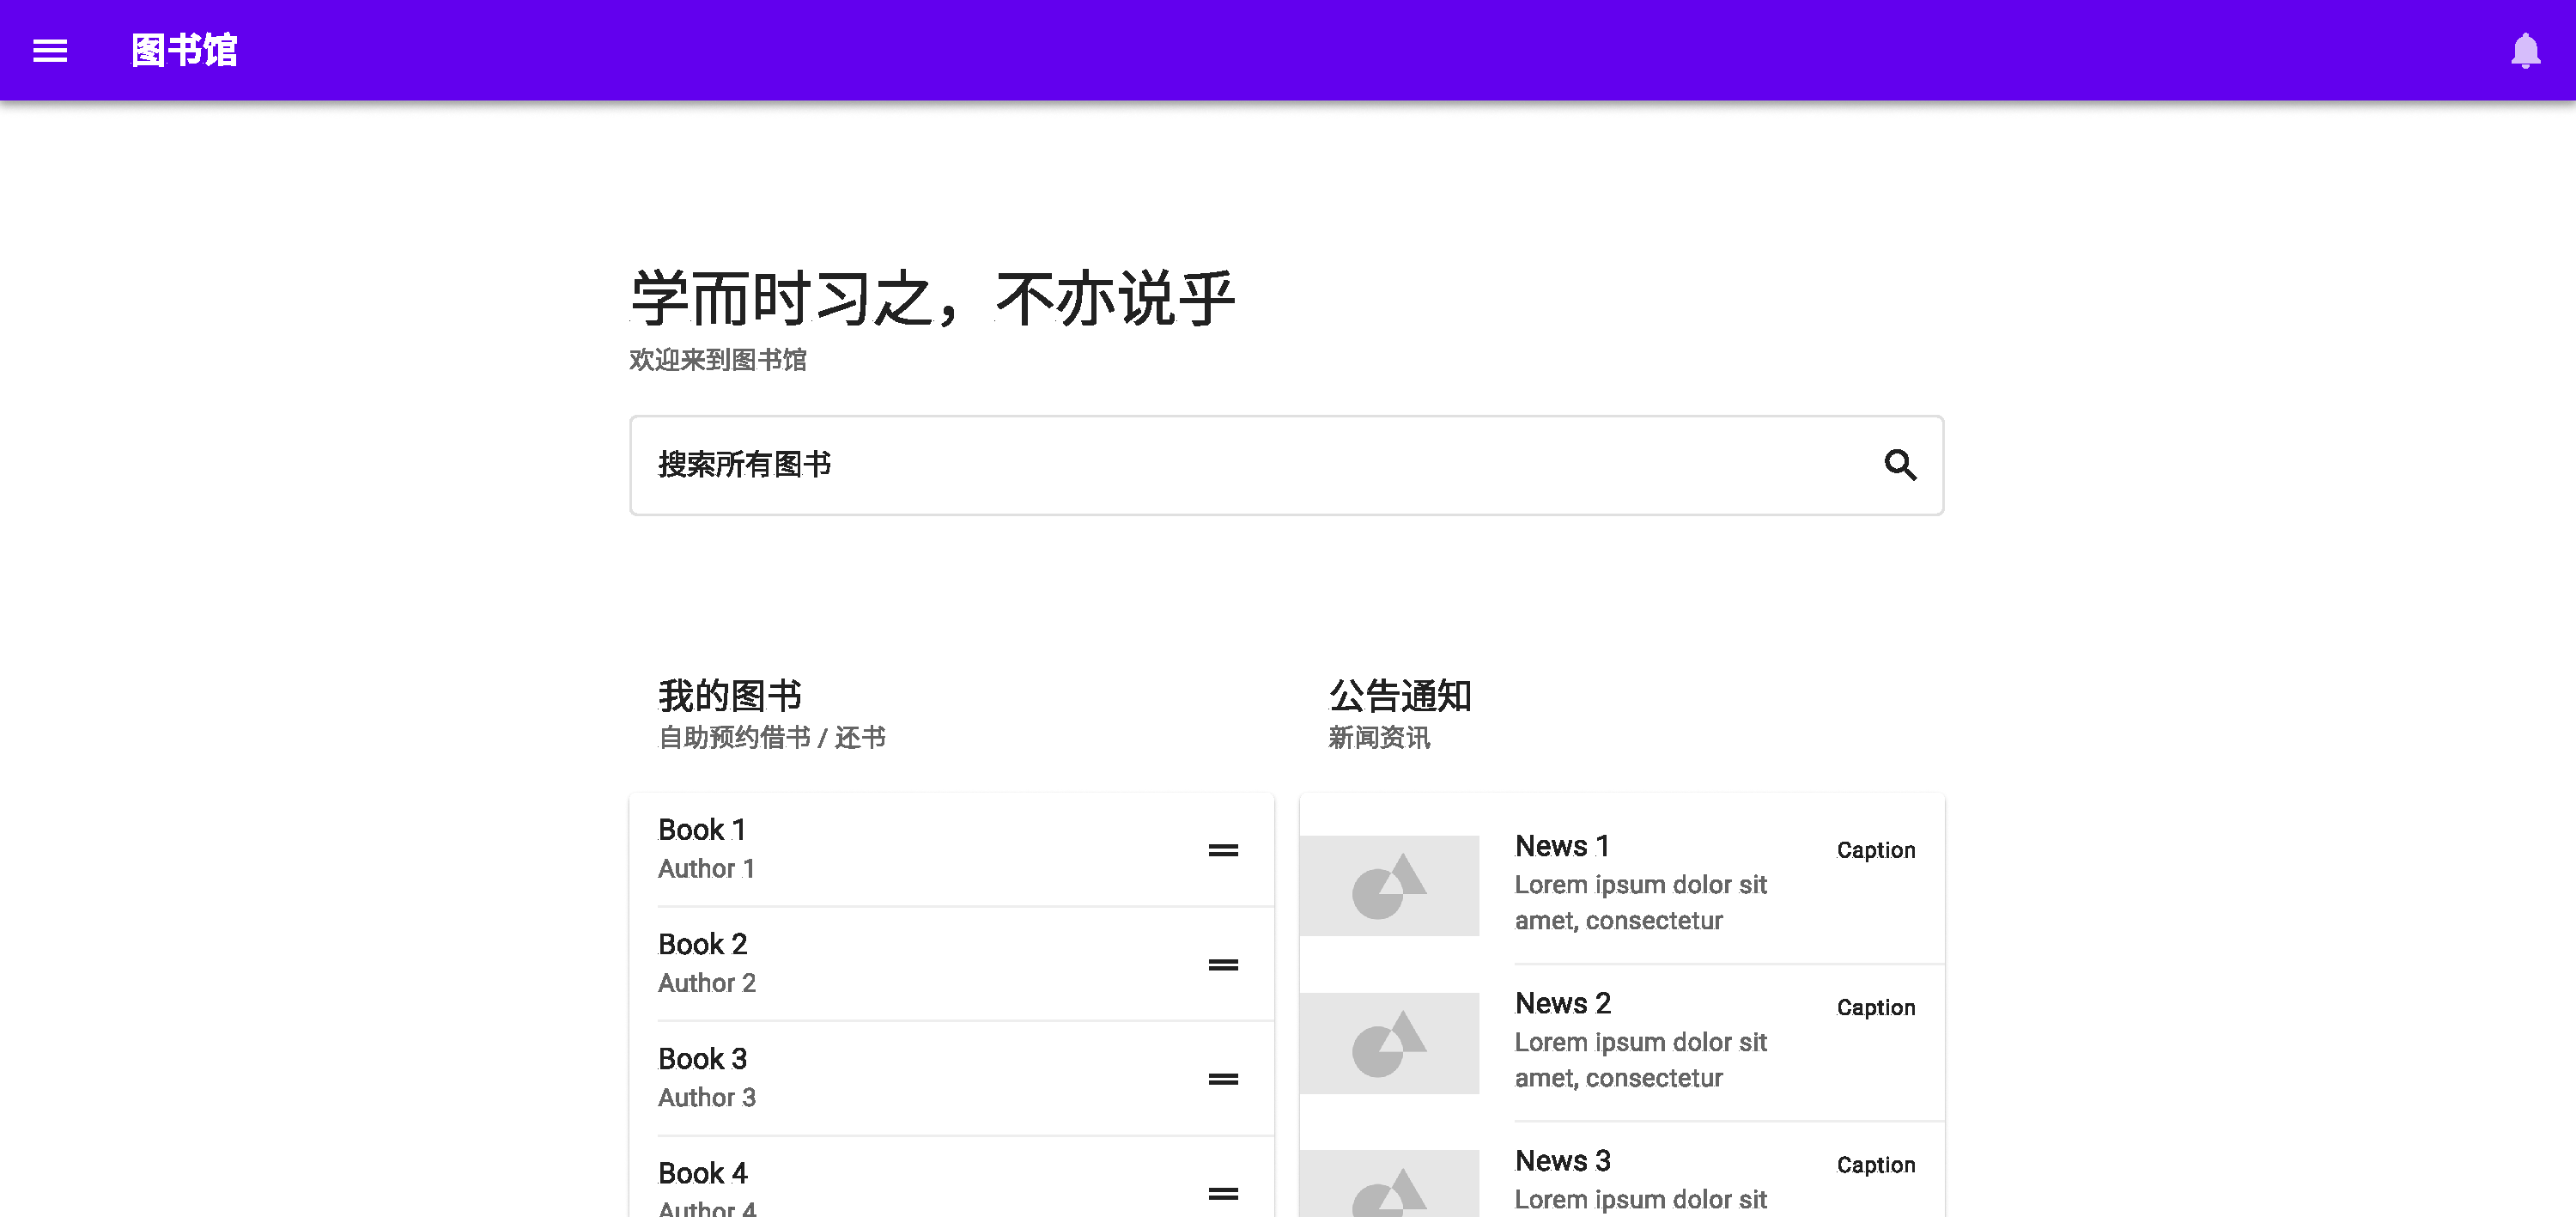
\includegraphics[width=\textwidth]{fig/library-interface.pdf}}
\textbf{图书馆检索界面}
\end{center}

\begin{center}
\shadowbox{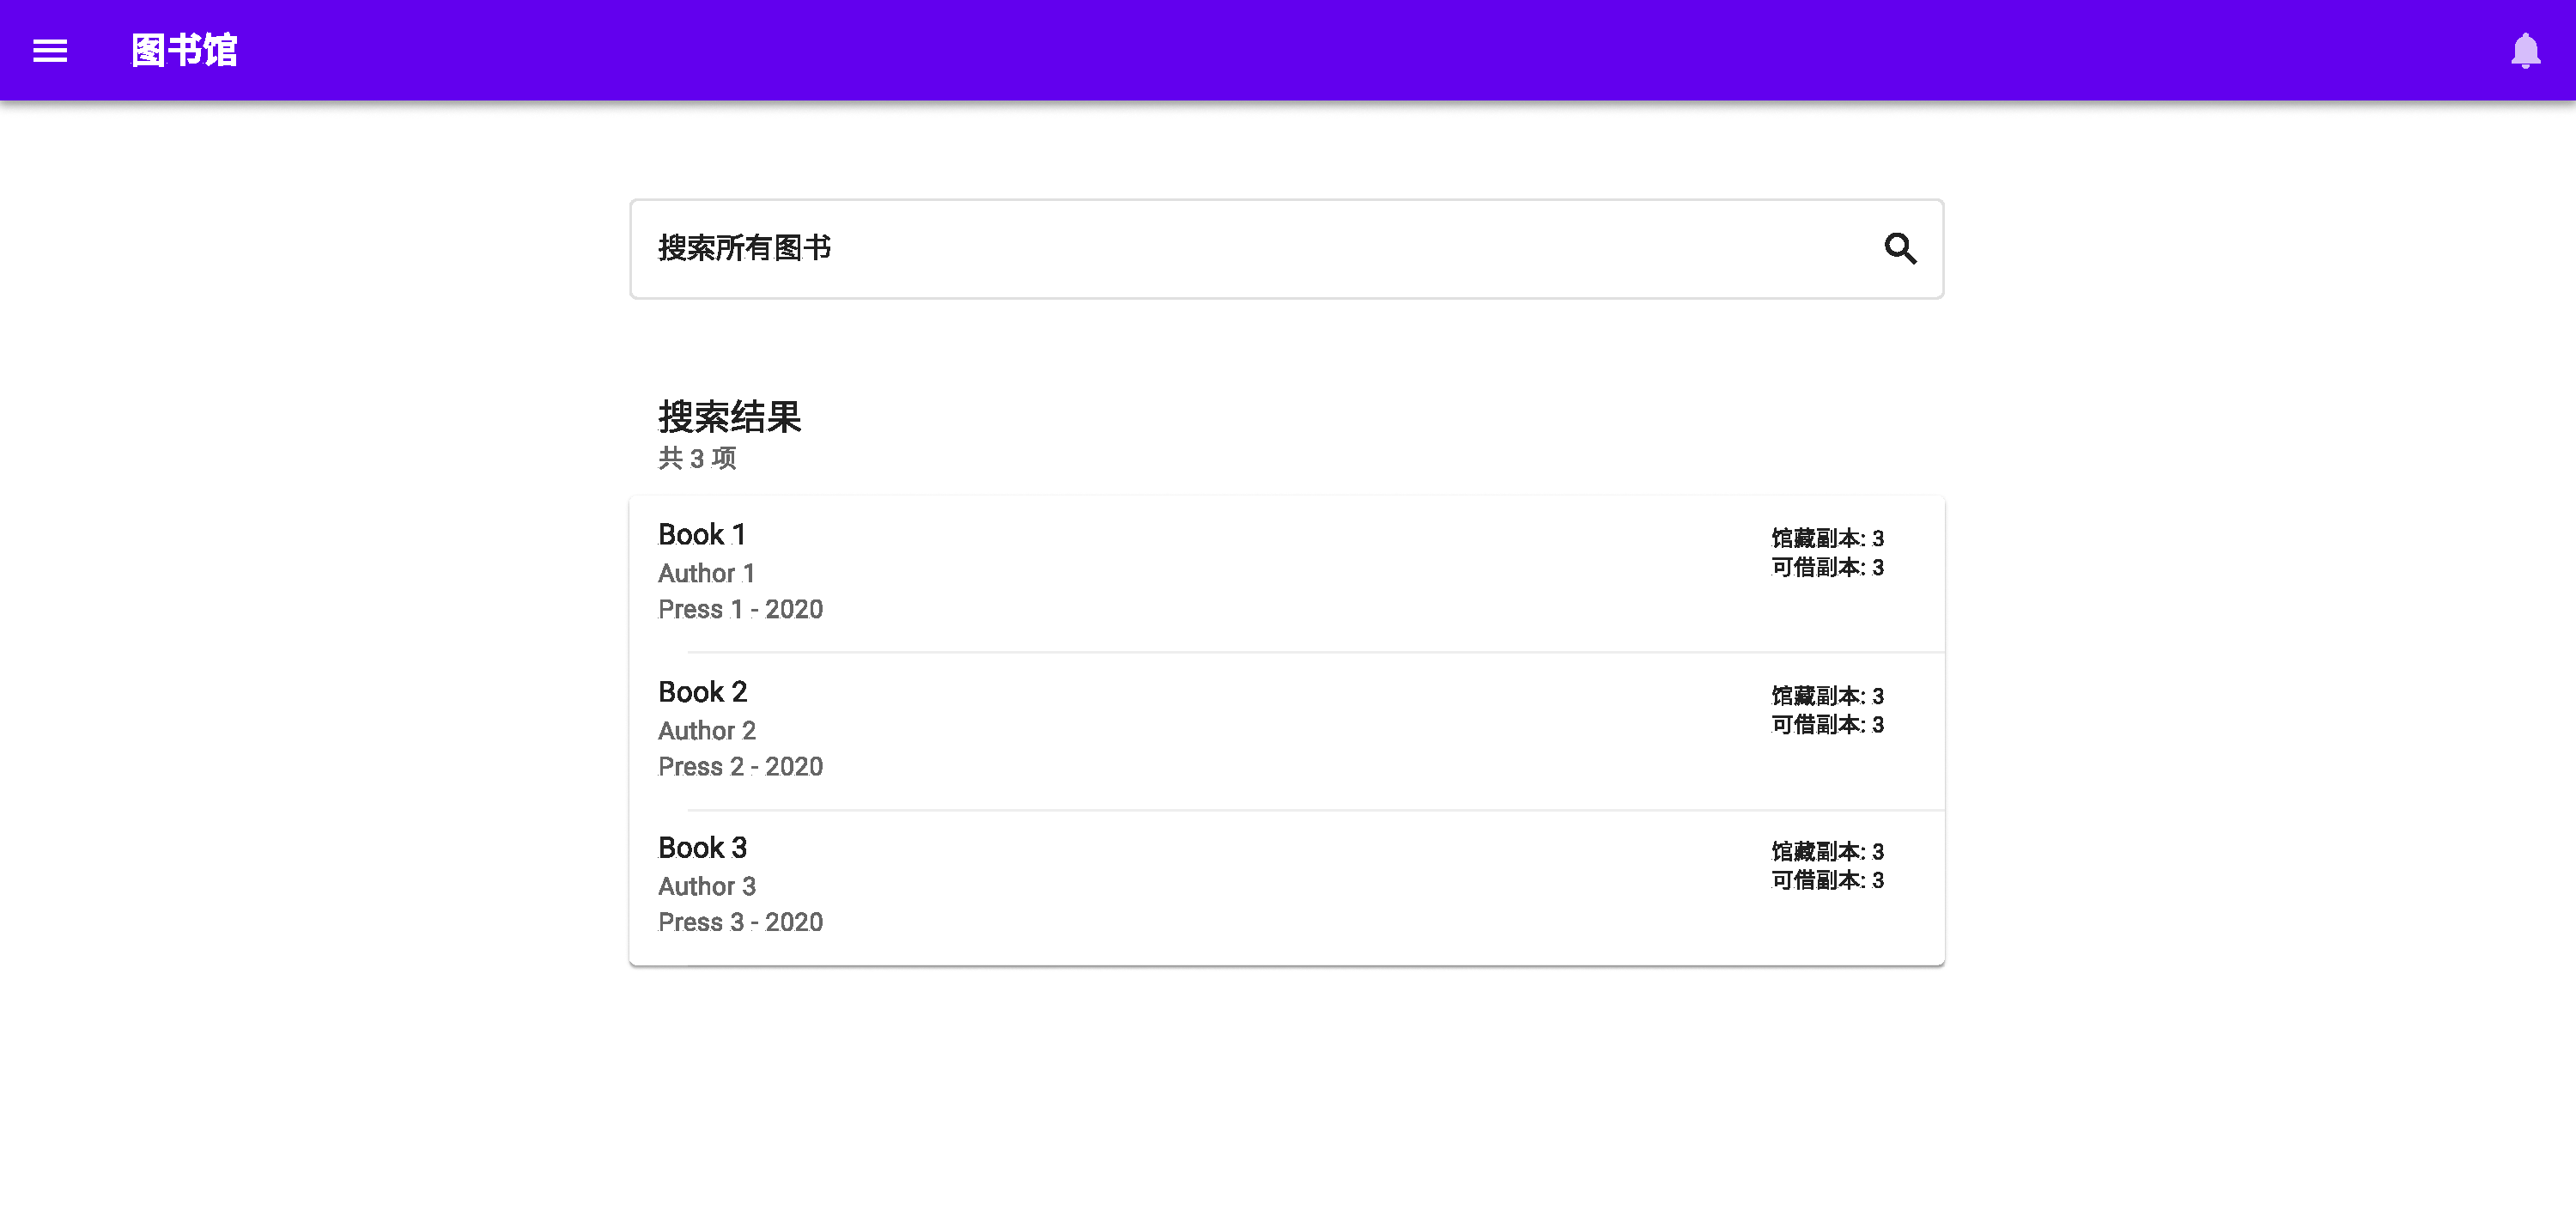
\includegraphics[width=\textwidth]{fig/library-search-interface.pdf}}
\textbf{检索结果页面}
\end{center}

\begin{center}
\shadowbox{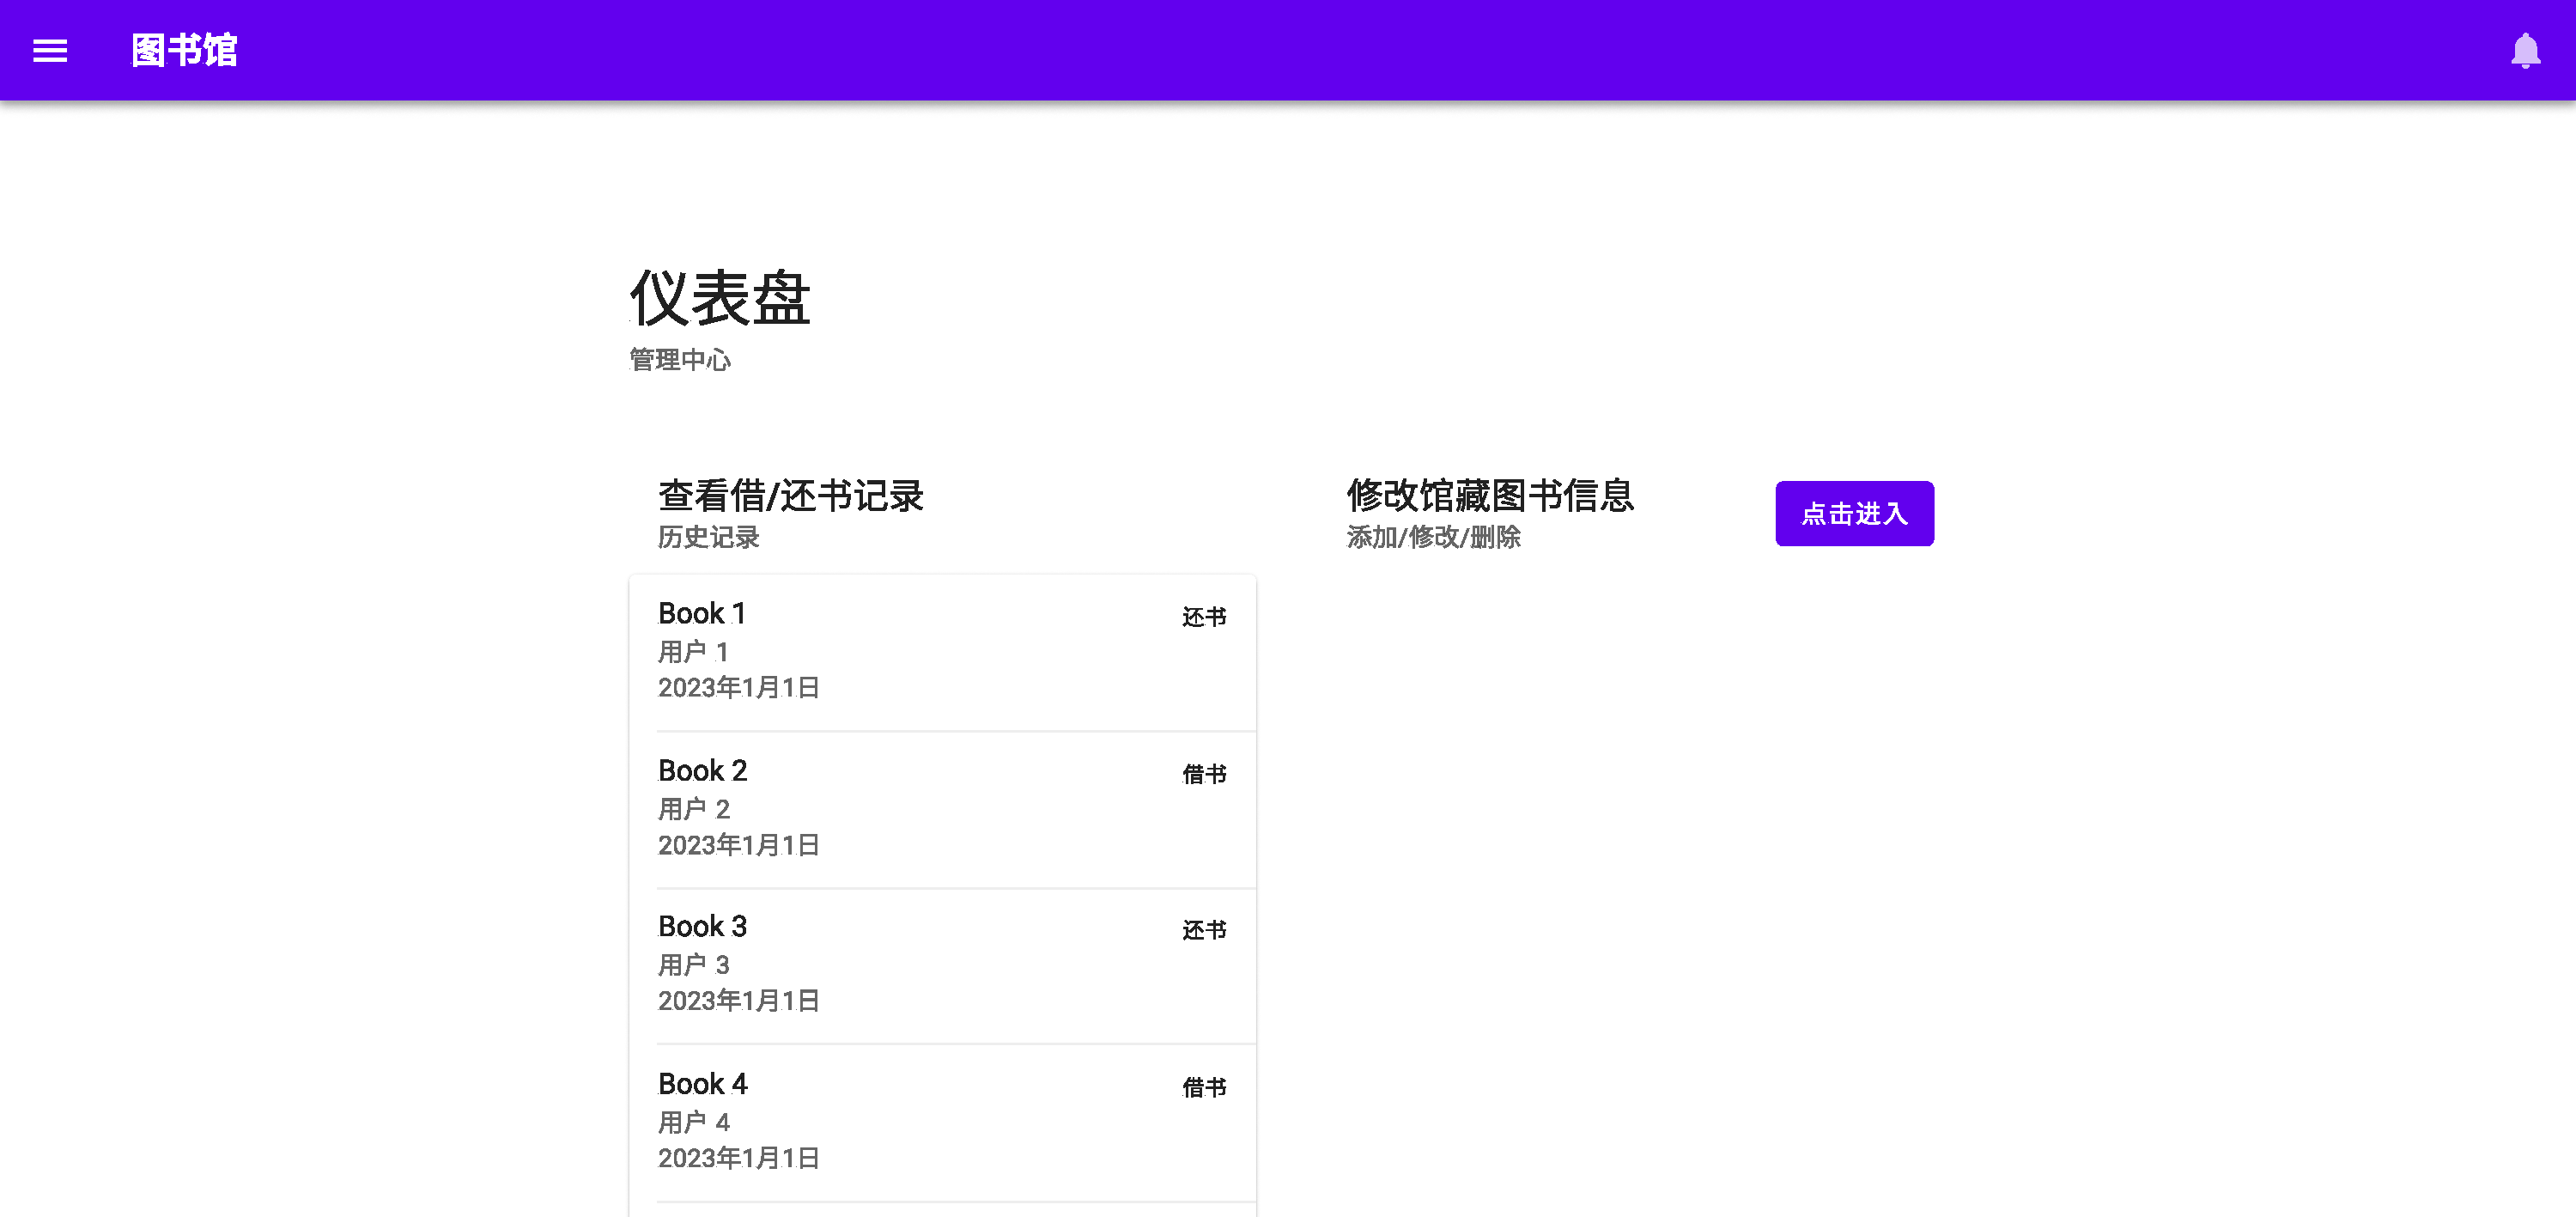
\includegraphics[width=\textwidth]{fig/library-dashboard-interface.pdf}}
\textbf{图书馆管理页面}
\end{center}

\subsubsection{模块流程图}
\begin{center}
    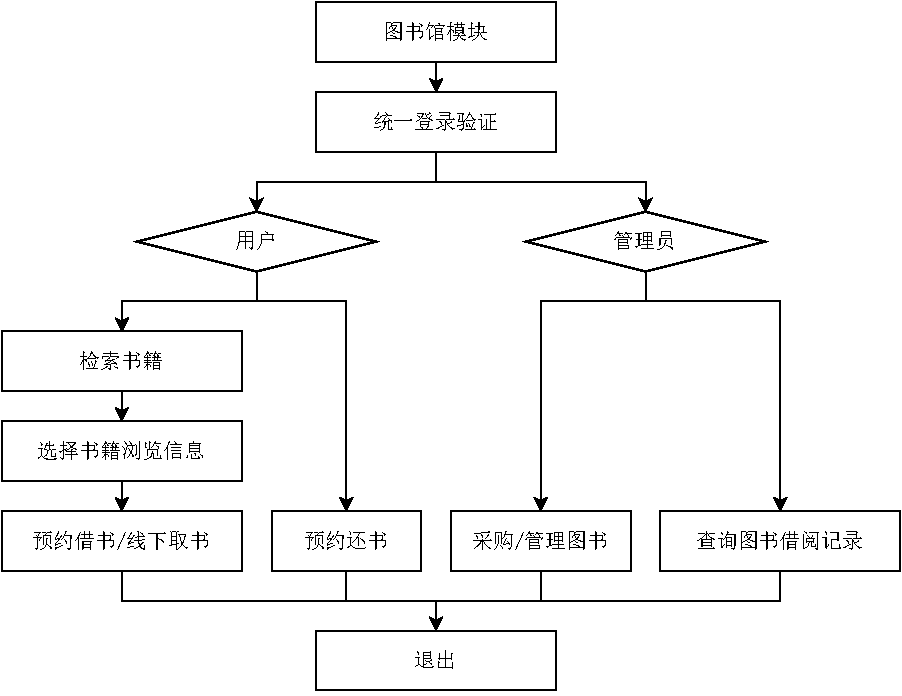
\includegraphics[width=0.8\textwidth]{fig/library-flowchart.pdf}
\end{center}

\newpage

\subsubsection{类分析}
\begin{enumerate}
    \item \textbf{实体类}


馆藏图书信息类:\texttt{LibraryBook}
\begin{table}[H]
  \centering
  \setlength{\tabcolsep}{6mm}{
    \begin{tabular}{ccccc}
    \hline
   序号& 名称  & 类型 & 约束  &备注 \\
    \hline
  1& \texttt{uuid} & \texttt{UUID} & & 图书编号 \\
  2&  \texttt{name}  & \texttt{String} & &书名 \\
  3&  \texttt{isbn}  & \texttt{String} &ISBN格式 &ISBN \\
  4&  \texttt{author} & \texttt{String} & &作者 \\
  5&  \texttt{press} & \texttt{String} & &出版社 \\
  6&  \texttt{description} & \texttt{String} & &简介 \\
  7&  \texttt{place} & \texttt{String} & &存放地点 \\
  8&  \texttt{status} & \texttt{enum}  & &出借状态 \\
    \hline
    \end{tabular}}
  \label{tab:addlabel}%
\end{table}%

用户信息类:\texttt{LibraryUser}

\begin{table}[H]
  \centering
   \setlength{\tabcolsep}{6mm}{
    \begin{tabular}{ccccc}
    \hline
    序号&名称    & 类型    & 约束&备注 \\
    \hline
   1& \texttt{userId} & \texttt{Integer}   & 9位数字&用户一卡通号 \\
   2& \texttt{userStatus} & \texttt{enum}  & &用户状态 \\
   3& \texttt{borrowed} & \texttt{Integer}   & 非负数&已借数量 \\
   4& \texttt{maxBorrow} & \texttt{Integer}   &非负数 &总共可借数量 \\
    \hline
    \end{tabular}}c 
  \label{tab:addlabel}%
\end{table}%


图书借阅记录类:\texttt{LibraryTransaction}

\begin{table}[H]
  \centering
  \setlength{\tabcolsep}{4mm}{
    \begin{tabular}{ccccc}
    \hline
   序号& 名称    & 类型    & 约束&备注 \\
    \hline
    1& \texttt{uuid} &  \texttt{UUID}  & &表内唯一标识信息 \\
    2& \texttt{bookUuid} &  \texttt{UUID}  & &书UUID \\
    3& \texttt{userId} &  \texttt{Integer}   & 9位数字&借阅者一卡通 \\
    4& \texttt{action} &  \texttt{enum}  & &借入/借出 \\
    5& \texttt{time}  &  \texttt{LocalDateTime} & &操作时间 \\
    \hline
    \end{tabular}}
\end{table}%


\item \textbf{服务类}

客户端:\texttt{LibraryClient}
    \begin{table}[H]
        \centering
        \setlength{\tabcolsep}{6mm}{
        \begin{tabular}{cccc}
        \hline
        序号&名称&方法&备注  \\
        \hline
        1&  检索图书 & \texttt{libFindBooks} & 用户检索书籍   \\
        2& 选择书籍 &  \texttt{libSelectBook}& 用户检索界面选择书籍浏览信息\\
        3& 预约借书 & \texttt{libBorrowBook} & 用户点击预约借书 \\
        4& 预约还书 & \texttt{libReturnBook}  & 用户预约还书  \\
        5& 图书入库 & \texttt{libAddBook} & 管理员采购书籍,图书入库\\
        6& 信息修改 & \texttt{libModifyInfo} & 管理员修改图书信息\\
        7& 查询借阅记录 & \texttt{libRecordQuery} & 管理员查询图书借阅记录    \\
        \hline
        \end{tabular}}
    \end{table}

\newpage

服务器端:\texttt{LibraryController}
    \begin{table}[H]
        \centering
        \setlength{\tabcolsep}{6mm}{
        \begin{tabular}{cccc}
        \hline
        序号&名称&方法&备注  \\
        \hline
        1&  返回检索信息 & \texttt{libGetBooks} & 依据用户的检索词返回对应的图书信息   \\
        2& 返回书籍信息 & \texttt{libGetBookInfo} & 根据用户选择返回对应的书籍具体信息 \\
        3& 状态修改& \texttt{libStatusModify} & 根据用户操作修改图书状态 \\
        4& 信息修改 & \texttt{libUpdateInfo} & 根据管理员修改的信息更新数据库\\
        5& 记录展示 & \texttt{libRecordShow} & 展示近期图书借阅记录\\
        \hline
        \end{tabular}}
    \end{table}
    


\end{enumerate}

\section{商店模块设计说明}
\subsection{模块背景}
用于为学生提供各种商品,并通过在线支付手段进行支付完成交易。
\subsection{需求分析}

\paragraph{用户角色和权限}
模块应支持不同的用户角色,如学生和商店管理员。不同角色应有不同的权限,例如学生可以浏览商品、下单购买,管理员可以管理用户、商品和订单。

\paragraph{用户认证和安全性}
用户需要登录账号后才能进入模块,确保信息安全。支付密码应该进行加密存储。同时,应该实施合适的安全措施,防止恶意攻击和数据泄露。

\paragraph{商品管理}
管理员应该能够添加、编辑和删除商品,并统计商品的销售情况。每个商品应该有名称、价格、库存数量、条形码等属性。商品应该有简洁的描述,以便用户更了解商品信息。

\paragraph{购物流程}
用户浏览商店,选择感兴趣的商品,并进行结算。结算应该能够显示商品交易金额、交易时间,并支持添加备注,然后进行线上支付。

\paragraph{数据统计和分析}
模块可以提供各种商品销量报告、热门商品统计、用户购买习惯等数据分析功能,帮助管理员做出更好的经营决策。

\paragraph{用户界面和体验}
用户界面应该友好、易用,并且能够突出商品特性和详细信息。响应式设计和良好的用户体验是至关重要的。

\paragraph{报错和异常处理}
模块应该能够处理用户可能遇到的各种错误和异常情况,如商品售罄、支付失败等问题,提供友好的错误提示和解决方案。

\subsection{系统设计}
\subsubsection{界面设计}

\begin{center}
\shadowbox{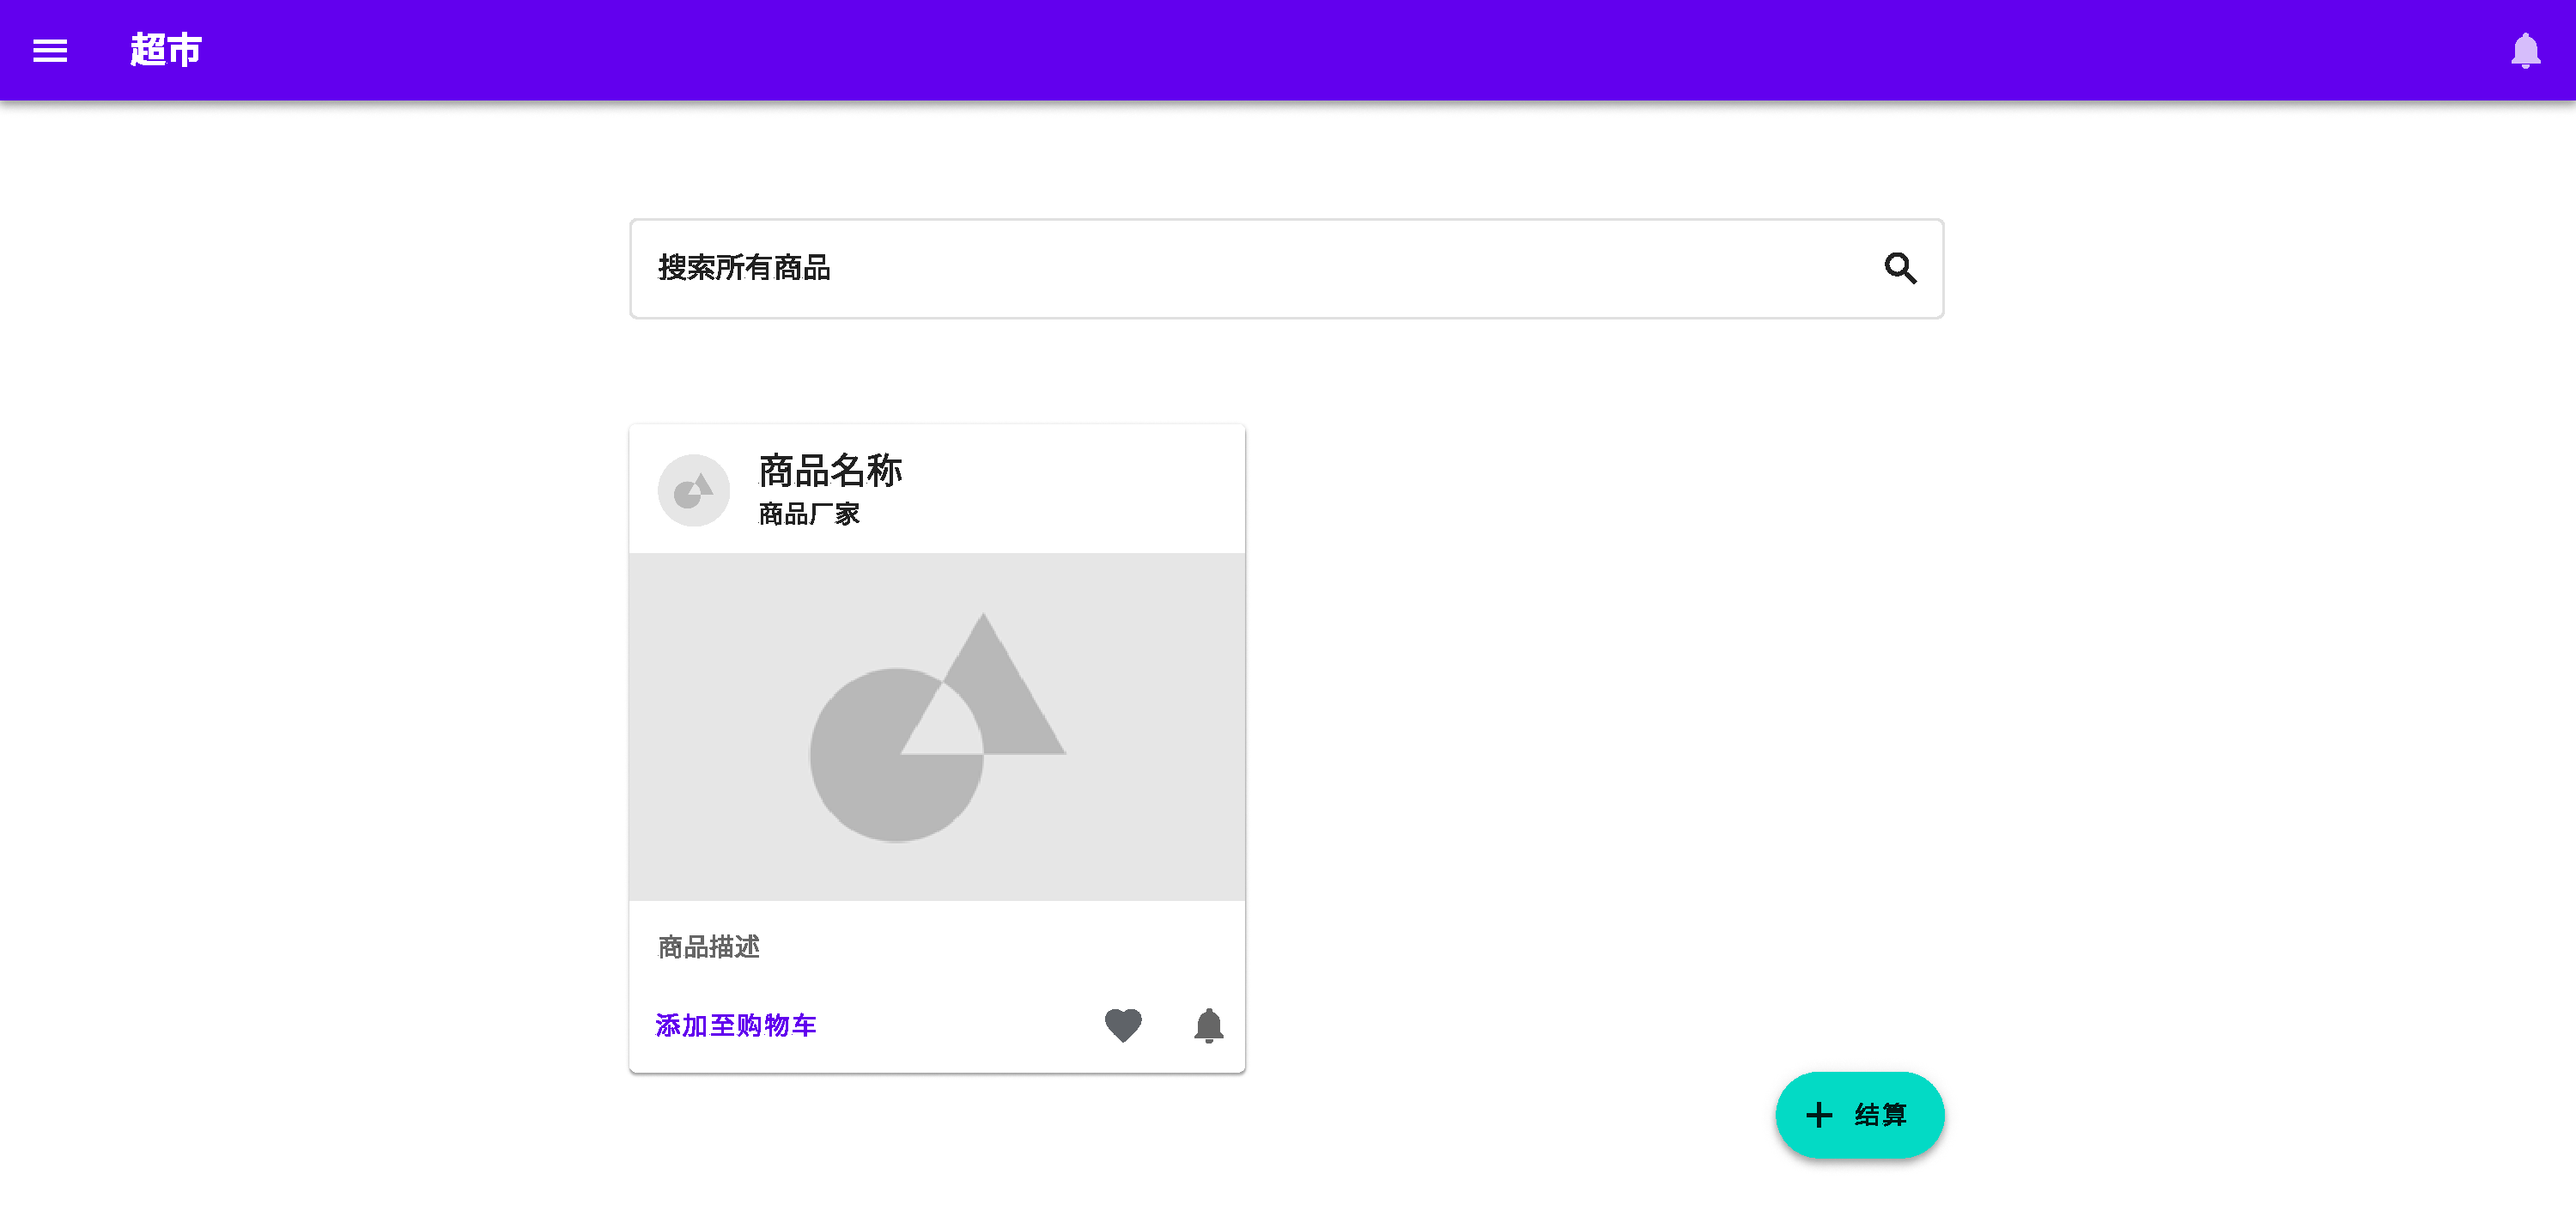
\includegraphics[width=\textwidth]{fig/store-interface.pdf}}
\textbf{商店选购页面}
\end{center}

\begin{center}
\shadowbox{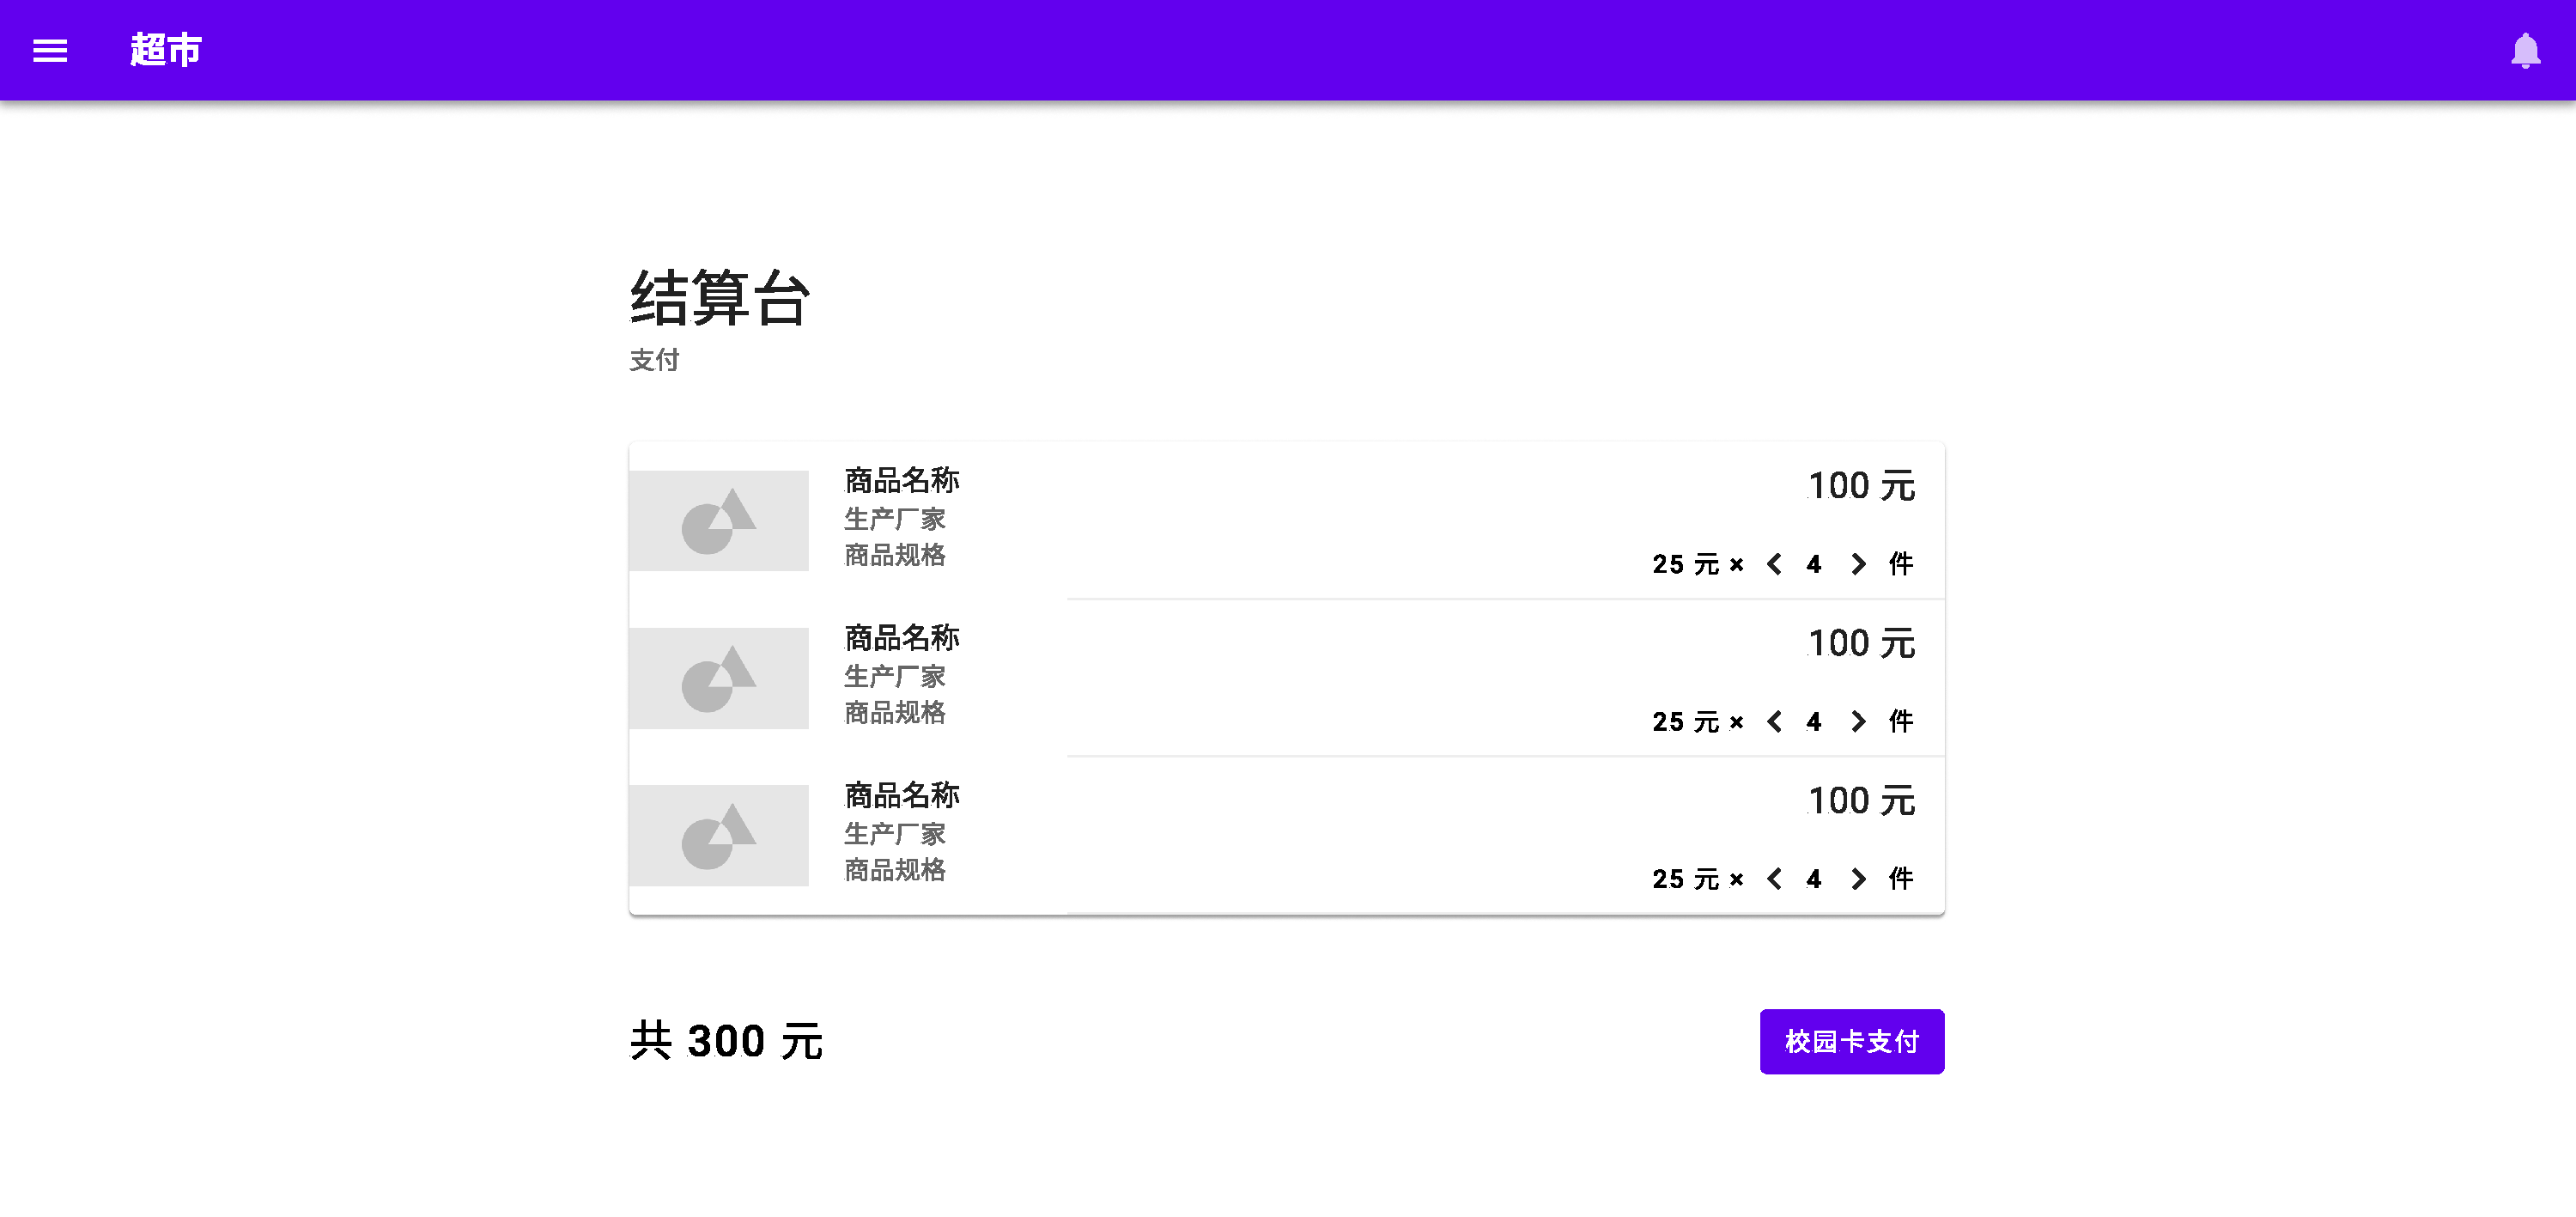
\includegraphics[width=\textwidth]{fig/store-check-interface.pdf}}
\textbf{商店结算页面}
\end{center}

\begin{center}
\shadowbox{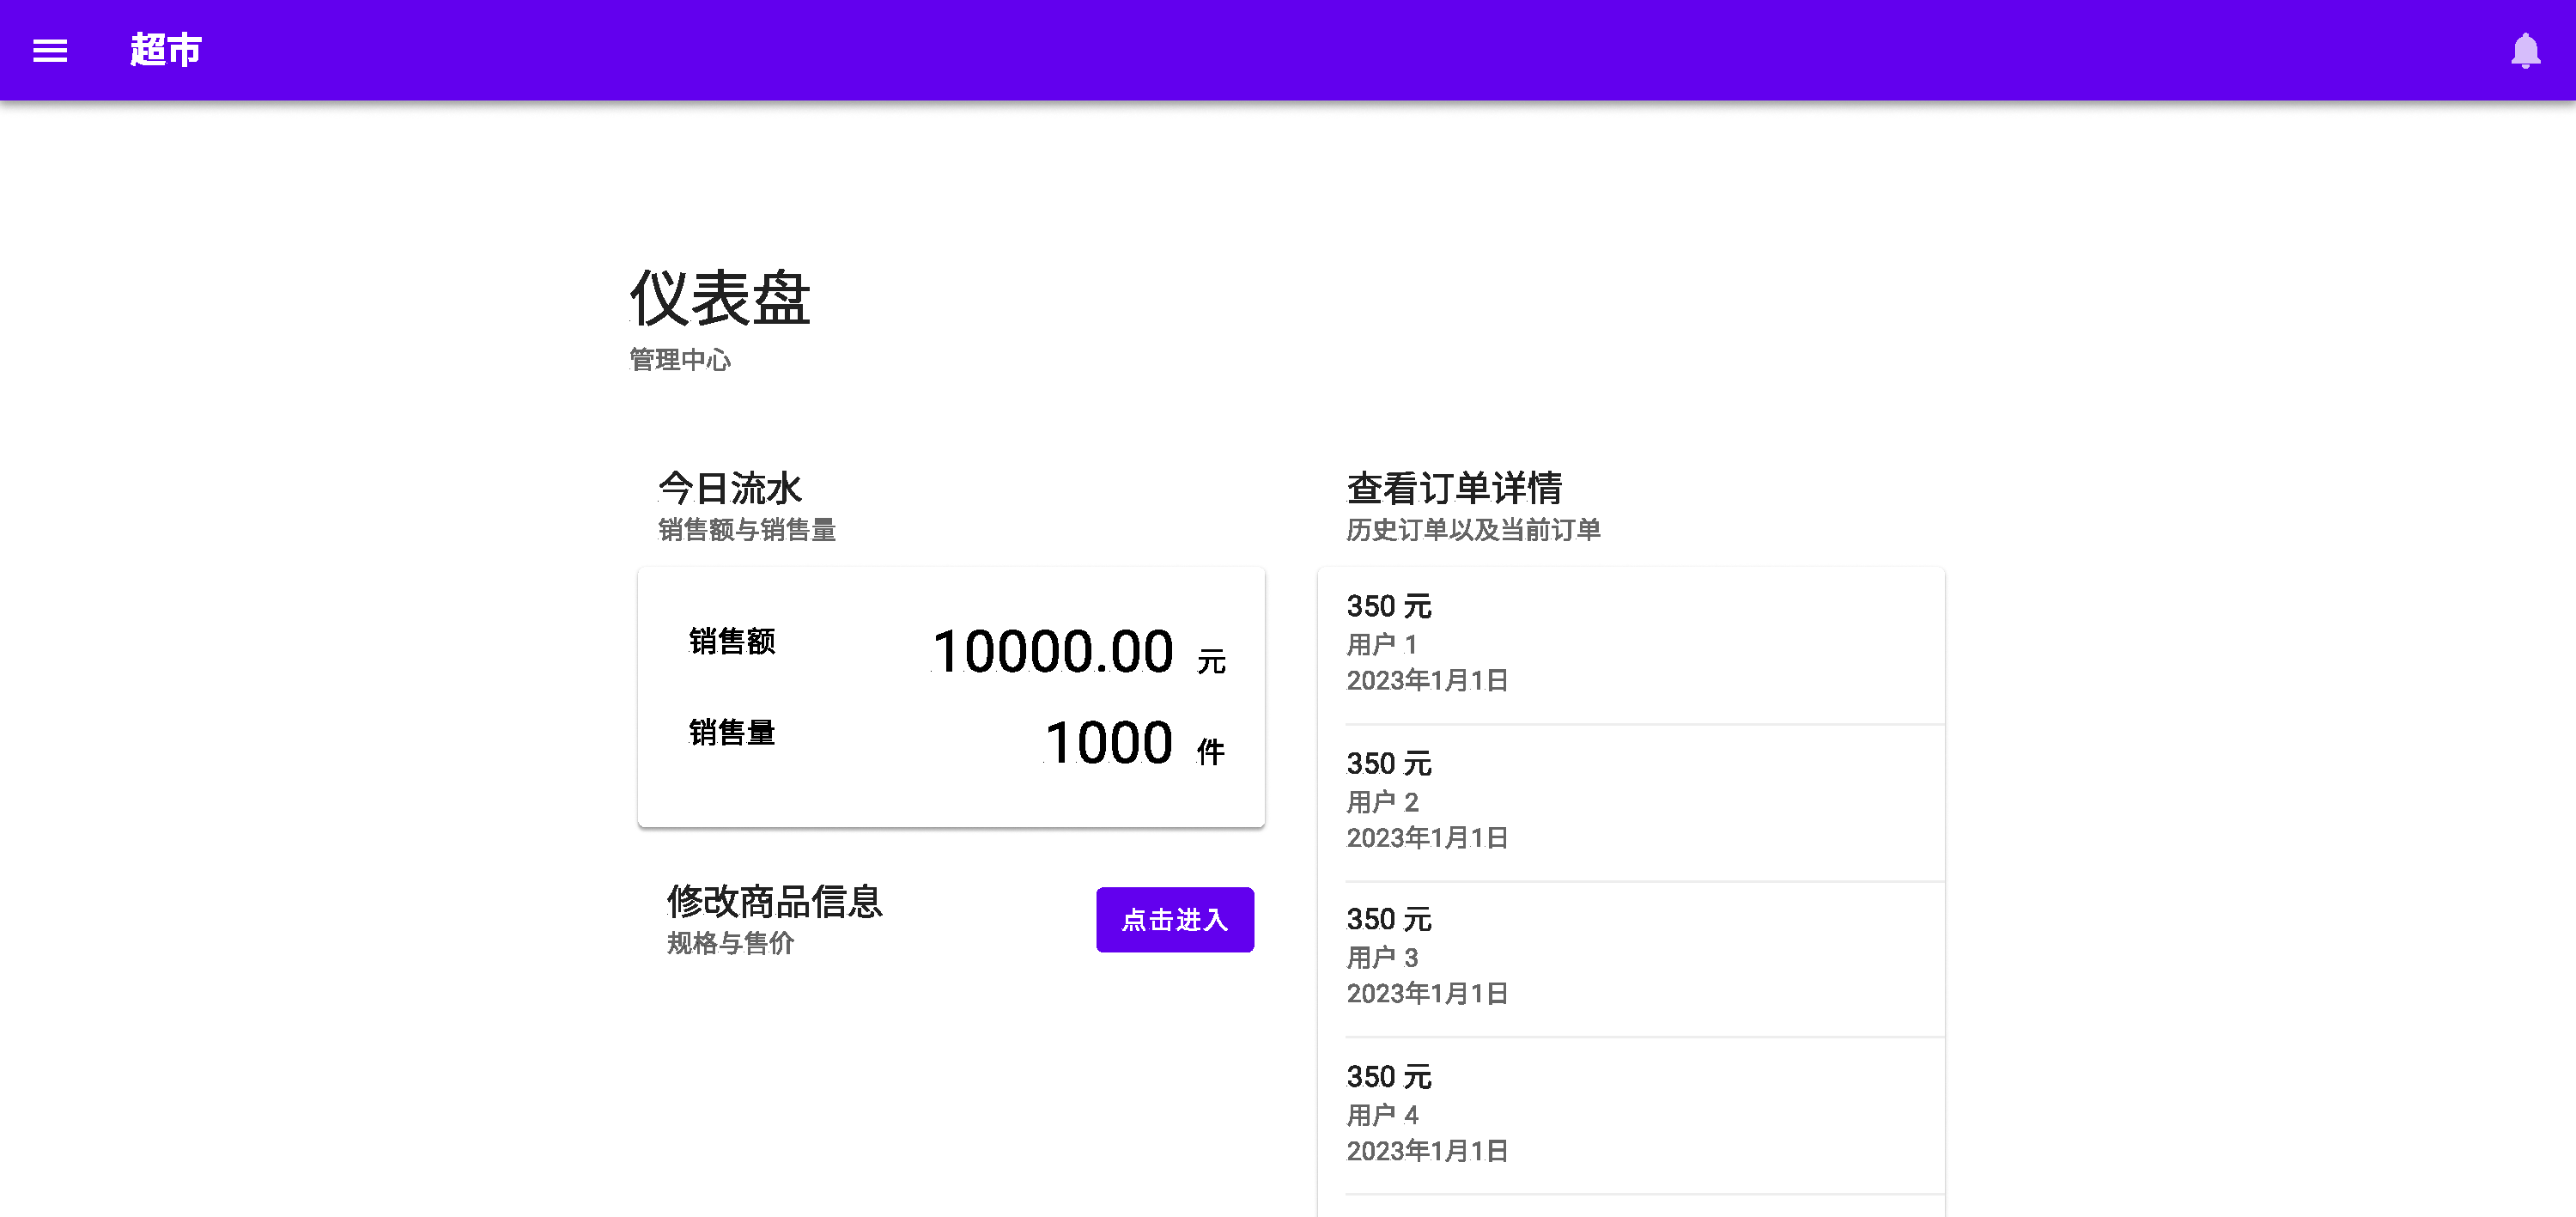
\includegraphics[width=\textwidth]{fig/store-dashboard-interface.pdf}}
\textbf{商店管理页面}
\end{center}

\subsubsection{模块流程图}

\begin{center}
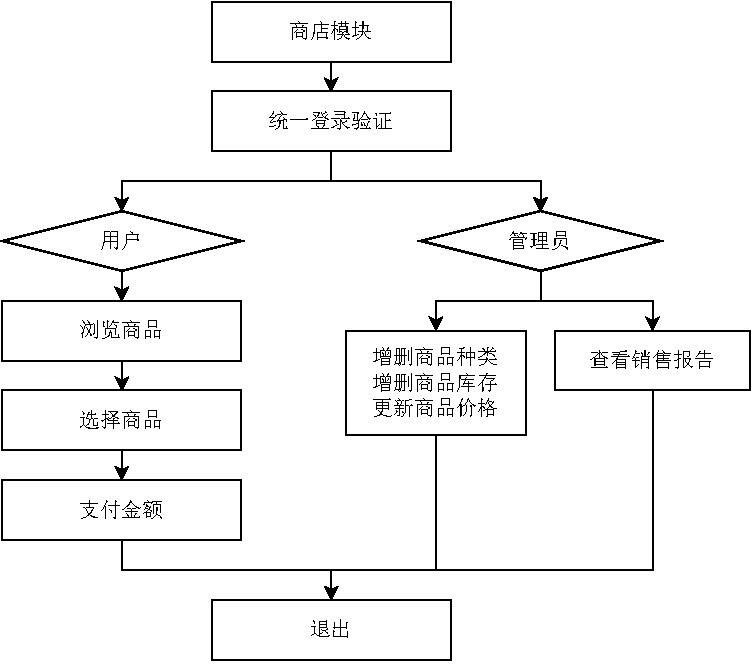
\includegraphics[width=0.7\textwidth]{fig/store-flowchart.pdf}
\end{center}

\newpage

\subsubsection{类分析}
\begin{enumerate}
    \item \textbf{实体类}


商品类:\texttt{StoreItem}
        \begin{table}[H]
        \centering
            \setlength{\tabcolsep}{6mm}{
                \begin{tabular}{ccccc}
                \hline
                序号    & 名称    & 类型    & 约束    & 备注\\
                \hline
                1 & \texttt{uuid} & \texttt{UUID}   &  & 商品编号\\
                2 & \texttt{name} & \texttt{String} & 不超过100个字符 & 商品名称\\
                3 & \texttt{price}  & \texttt{Integer} & 非负数 & 商品金额\\
                4 & \texttt{barcode}  & \texttt{String} & 13个字符 & 商品条形码\\
                5  & \texttt{stock}   & \texttt{Integer} & 非负数 & 商品库存数量\\
                6 &\texttt{description}  & \texttt{String} &  &商品信息描述\\
                \hline
        \end{tabular}}
        \end{table}
        
商品交易记录类:\texttt{StoreTransaction} 

\begin{table}[H]
  \centering
  \setlength{\tabcolsep}{3mm}{
    \begin{tabular}{ccccc}
    \hline
    序号    & 名称    & 类型    & 约束    & 备注\\
    \hline
    1 & \texttt{uuid} & \texttt{UUID}   & & 交易编号\\
    2 & \texttt{itemUuid} & \texttt{UUID} & & 交易中的商品编号\\
    3 & \texttt{itemPrice} & \texttt{Integer}   & 非负数 & 交易中的商品单价\\
    4 & \texttt{amount} & \texttt{Integer} & 非负数 & 交易中的商品数量\\
    5 & \texttt{cardNumber} & \texttt{Integer} & 9位数字 & 交易关联一卡通号\\
    6 & \texttt{time} & \texttt{LocalDateTime}   &  & 交易的时间\\
    7 & \texttt{remark} & \texttt{String} & & 交易的备注信息\\
    \hline
    \end{tabular}}
\end{table}
\item \textbf{服务类}

{客户端:\texttt{StoreClient}
    \begin{table}[H]
        \centering
            \setlength{\tabcolsep}{6mm}{
                \begin{tabular}{cccc}
                \hline
                序号    & 名称    & 方法    & 备注\\
                \hline
                1 & 查找 & \texttt{retrieveItem} & 查找要购买的商品\\
                2 & 选择 & \texttt{selectItem} & 选择要购买的商品\\
                3 & 移除 & \texttt{removeItem} & 从购物车中移除商品\\
                4 & 结算  & \texttt{settle} & 结算选择的商品总金额\\
                5 & 支付  & \texttt{pay} & 输入密码进行支付\\
                6 & 新增商品   & \texttt{createItem} & 管理员添加新的商品\\
                7 & 删除商品  & \texttt{deleteItem} & 管理员删除商品\\
                8 & 更新信息  & \texttt{updateInfo} & 管理员更新商品信息(价格、库存等)\\
                9 & 查看报告  & \texttt{getReport} & 管理员查看销售报告\\
                \hline
        \end{tabular}}
        \end{table}

\newpage
        
服务器端:\texttt{StoreController}
    \begin{table}[H]
        \centering
            \setlength{\tabcolsep}{6mm}{
                \begin{tabular}{cccc}
                \hline
                序号    & 名称    & 方法    & 备注\\
                \hline
                1 & 查找 & \texttt{getItem} & 根据关键词查找商品,并返回匹配的商品\\
                2 & 记录 & \texttt{selectItem} & 记录选择的商品信息\\
                3 & 移除 & \texttt{removeItem} & 从记录中移除某个商品\\
                4 & 结算  & \texttt{settle} & 结算选择的商品总金额\\
                5 & 支付  & \texttt{pay} & 根据账号和密码进行支付\\
                6 & 新增商品   & \texttt{createItem} & 管理员添加新的商品\\
                7 & 删除商品  & \texttt{deleteItem} & 管理员删除商品\\
                8 & 更新信息  & \texttt{updateInfo} & 管理员更新商品信息(价格、库存等)\\
                9 & 查看报告  & \texttt{getReport} & 生成销售报告\\
                \hline
        \end{tabular}}
        \end{table}}
    


\end{enumerate}

\section{\texttt{TODO:} 其他选做模块}

\section{公共模块设计说明}
\subsection{消息信息模型}

\subsubsection{\texttt{Request}}

\begin{table}[H]
  \centering
  \setlength{\tabcolsep}{10mm}{
    \begin{tabular}{ccc}
    \hline
    名称    & 类型    & 备注\\
    \hline
    \texttt{uri} & \texttt{String}   & 请求资源唯一标识符 \\
    \texttt{params} & \texttt{Map<String, String>} & 请求参数 \\
    
    \texttt{session} & \texttt{Session}  & 由服务端维护的 Session 状态 \\
    \hline
    \end{tabular}}
\end{table}

\subsubsection{\texttt{Response}}

\begin{table}[H]
  \centering
  \setlength{\tabcolsep}{10mm}{
    \begin{tabular}{ccc}
    \hline
    名称    & 类型    & 备注\\
    \hline
    \texttt{status} & \texttt{String}   & 响应状态 \\
    \texttt{message} & \texttt{String} & 响应信息 \\
    \texttt{data} & \texttt{Object}  & 响应体 \\

    \texttt{session} & \texttt{Session}  & 对服务端 Session 状态更新 \\
    \hline
    \end{tabular}}
\end{table}

\subsection{用户信息模型}
\subsection{工具类}
\subsubsection{数据库工具类}

\begin{table}[H]
  \centering
  \setlength{\tabcolsep}{6mm}{
    \begin{tabular}{ccc}
    \hline
    名称    & 说明    & 备注\\
    \hline
    \texttt{init()} & 完成配置初始化 & 返回 \texttt{org.hibernate.Session} 对象 \\
    \hline
    \end{tabular}}
\end{table}

\subsubsection{密码工具类}

\begin{table}[H]
  \centering
  \setlength{\tabcolsep}{6mm}{
    \begin{tabular}{ccc}
    \hline
    名称    & 说明    & 备注\\
    \hline
    \texttt{encoder()} & 返回 \texttt{Argon2PasswordEncoder} & \\
    \texttt{hash(password)} & 返回 hash 后的密码 & 使用 \texttt{Argon2} 算法 \\
    \texttt{verify(password, hashed)} & 验证密码 &  \\
    \hline
    \end{tabular}}
\end{table}

% \subsection{Message}
% \subsection{User}
% \subsection{数据库工具类DbHelper}
% \subsection{数据存取类DAO}
% \subsection{工具类}
% \subsection{其他类}


\section{网络模块设计说明}

为方便开发以及性能,我们采用 Netty 库作为 Socket 实现,客户端与服务端的数据交换封装为 \texttt{Request} 与 \texttt{Response} 实现,通过扩展 \texttt{ChannelInboundHandlerAdapter} 实现数据发送与接收,并使用 \texttt{Gson} 库进行数据序列化。

\subsection{Socket}
\subsubsection{客户端}

\subsubsection{服务器端 \texttt{NettyServer}}

\begin{table}[H]
  \centering
  \setlength{\tabcolsep}{6mm}{
    \begin{tabular}{ccc}
    \hline
    名称    & 说明    & 备注\\
    \hline
    \texttt{NettyServer(port)} & 初始化相关配置 & 传入端口 \\
    \texttt{run(router, database)} & 启动服务器 & 传入 \texttt{Router} 与数据库 \texttt{Session} \\
    \hline
    \end{tabular}}
\end{table}

\begin{lstlisting}
NettyServer server = new NettyServer(9090);
server.run(router);
\end{lstlisting}

\subsection{输入输出流}
\subsubsection{读取输入}

借助 \texttt{Netty} 提供的 \texttt{ChannelPipeline} 和 \texttt{ChannelInboundHandlerAdapter} 等工具,可方便地定义流的处理方式。

\begin{lstlisting}
EventLoopGroup bossGroup = new NioEventLoopGroup();
EventLoopGroup workerGroup = new NioEventLoopGroup();
try {
    ServerBootstrap b = new ServerBootstrap();
    b.group(bossGroup, workerGroup)
            .channel(NioServerSocketChannel.class)
            .childHandler(new ChannelInitializer<SocketChannel>() {
                @Override
                public void initChannel(@NonNull SocketChannel ch) {
                    ch.pipeline().addLast(new JsonObjectDecoder()).addLast(new NettyHandler(router));
                }
            })
            .option(ChannelOption.SO_BACKLOG, 128)
            .childOption(ChannelOption.SO_KEEPALIVE, true);
    ChannelFuture f = b.bind(port).sync();
    f.channel().closeFuture().sync();
} finally {
    workerGroup.shutdownGracefully();
    bossGroup.shutdownGracefully();
}
\end{lstlisting}

\begin{lstlisting}
@Override
public void channelRead(@NonNull ChannelHandlerContext ctx, @NonNull Object msg) {
    ByteBuf in = (ByteBuf) msg;
    try {
        log.info("[{}] Received: {}", ctx.channel().id(), in.toString(CharsetUtil.UTF_8));
        Request request = gson.fromJson(in.toString(CharsetUtil.UTF_8), Request.class);
        request.setSession(session);
        if (!router.hasRoute(request.getUri())) {
            log.info("[{}] Route not found: {}", ctx.channel().id(), request.getUri());
            sendResponse(ctx, Response.Common.notFound());
            return;
        } else if (!session.permission(router.getRole(request.getUri()))) {
            log.info("[{}] Permission denied: {}", ctx.channel().id(), request.getUri());
            sendResponse(ctx, Response.Common.permissionDenied());
            return;
        }
        Response response = router.invoke(request);
        if (response.getSession() != null) {
            log.info("[{}] Session updated: {}", ctx.channel().id(), response.getSession());
            session = response.getSession();
        }
        sendResponse(ctx, response);
    } catch (Exception e) {
        log.error("[{}] Exception: {}", ctx.channel().id(), e.getMessage());
    } finally {
        ReferenceCountUtil.release(msg);
    }
}
\end{lstlisting}


\subsubsection{发送输出}

\begin{lstlisting}
private void sendResponse(ChannelHandlerContext ctx, Response response) {
    ctx.writeAndFlush(Unpooled.copiedBuffer(gson.toJson(response), CharsetUtil.UTF_8));
}
\end{lstlisting}

\section{多线程模块设计说明}

对于 UI,Compose 库自行管理渲染线程,无需编写相关多线程代码。

对于 Socket,使用 \texttt{Netty} 内置的 \texttt{NioEventLoopGroup},包括了线程池与 \texttt{NIO} 的使用,在独立线程中处理 Socket 连接。

\section{数据库设计说明}
\subsection{元数据}

共有14个数据库,名称以及说明如下表:

\begin{table}[H]
  \centering
  \setlength{\tabcolsep}{10mm}{
    \begin{tabular}{cc}
    \hline
    名称    & 说明 \\
    \hline
    \texttt{user}  & 存储用户信息 \\
    \texttt{student} & 存储学生学籍信息 \\
    \texttt{major} & 存储专业查询表\\
    \texttt{school} & 存储学院查询表 \\
    \texttt{accounting} & 存储财务账户信息 \\
    \texttt{card\_transaction} & 存储财务交易记录\\
    \texttt{course} & 存储课程信息\\
    \texttt{class} & 存储教学班信息\\
    \texttt{selected\_class} & 存储选课信息\\
    \texttt{library\_book} & 存储图书馆馆藏书目信息\\
    \texttt{library\_user} & 存储图书馆用户信息\\
    \texttt{library\_transaction} & 存储图书馆借还书记录\\
    \texttt{store\_item} & 存储商品信息\\
    \texttt{store\_transaction} & 存储商店交易记录\\
    \hline
    \end{tabular}}
\end{table}


\subsection{表设计}

\subsubsection{\texttt{user}表}

\texttt{user}表用于存储所有用户的信息,包括学生、教职员工等。

\begin{table}[H]
  \centering
  \setlength{\tabcolsep}{10mm}{
    \begin{tabular}{cccc}
    \hline
    字段    & 类型 & 约束   & 说明\\
    \hline
    \texttt{card\_number} & \texttt{INT} & 9位数字 & 存一卡通号\\
    \texttt{password} & \texttt{VARCHAR} & & 存储处理过的密码\\
    \texttt{name}  & \texttt{VARCHAR} & & 存储用户姓名\\
    \texttt{gender} & \texttt{ENUM} &  & 存储用户性别\\
    \texttt{phone}  & \texttt{VARCHAR} &  & 存储用户手机号\\
    \texttt{email}  & \texttt{VARCHAR} &  & 存储用户邮箱\\
    \texttt{role}  & \texttt{VARCHAR} &  & 存储用户角色\\
    \hline
    \end{tabular}}
\end{table}

\subsubsection{\texttt{student}表}

\texttt{student}表用于存储学生学籍信息。

\begin{table}[H]
  \centering
  \setlength{\tabcolsep}{4mm}{
    \begin{tabular}{cccc}
    \hline
    字段    & 类型 &约束   & 说明\\
    \hline
    \texttt{card\_number} & \texttt{INT} & 9位数字 & 存一卡通号\\
    \texttt{student\_number} & \texttt{VARCHAR} & 8位数字 & 存学号 \\
    \texttt{major} & \texttt{INT} &  & 专业编号 \\
    \texttt{school} & \texttt{INT}  & & 学院编号 \\
    \texttt{status} & \texttt{ENUM} & & 学籍状态 \\
    \texttt{enrollment} & \texttt{DATE} & & 入学日期 \\
    \texttt{birth\_place} & \texttt{VARCHAR} & & 籍贯 \\
    \texttt{political\_status} & \texttt{ENUM} & & 政治面貌\\
    \hline
    \end{tabular}}
\end{table}

\subsubsection{\texttt{major}表}

\texttt{major}表用于存储专业编号对应的专业名称。

\begin{table}[H]
  \centering
  \setlength{\tabcolsep}{10mm}{
    \begin{tabular}{cccc}
    \hline
    字段    & 类型 &约束   & 说明\\
    \hline
    \texttt{major\_number} & \texttt{INT}  & & 专业编号\\
    \texttt{major\_name} & \texttt{VARCHAR} & & 对应名称\\
    \hline
    \end{tabular}}
\end{table}

\subsubsection{\texttt{school}表}

\texttt{school}表用于存储学院编号对应的学院名称。

\begin{table}[H]
  \centering
  \setlength{\tabcolsep}{10mm}{
    \begin{tabular}{cccc}
    \hline
    字段    & 类型  &约束  & 说明\\
    \hline
    \texttt{school\_number} & \texttt{INT} &  & 学院编号\\
    \texttt{school\_name} & \texttt{VARCHAR} & & 对应名称\\
    \hline
    \end{tabular}}
\end{table}

\subsubsection{\texttt{accounting}表}

\texttt{accounting}表用于存储所有人一卡通的余额以及状态。

\begin{table}[H]
  \centering
  \setlength{\tabcolsep}{4mm}{
    \begin{tabular}{cccc}
    \hline
    字段    & 类型  & 约束  & 说明\\
    \hline
    \texttt{card\_number} & \texttt{INT} & 9位数字 & 存一卡通号\\
    \texttt{balance} & \texttt{INT}  & 非负数 & 存卡内余额(以分为单位) \\
    \texttt{card\_status} & \texttt{ENUM} & & 存一卡通状态\\
    \hline
    \end{tabular}}
\end{table}

\subsubsection{\texttt{card\_transaction}表}

\texttt{card\_transaction}表用于存储一卡通的交易信息。

\begin{table}[H]
  \centering
  \setlength{\tabcolsep}{4mm}{
    \begin{tabular}{cccc}
    \hline
    字段    & 类型 & 约束   & 说明 \\
    \hline
    \texttt{uuid}  & \texttt{UUID} & & 表内唯一标识信息,用作主键\\
    \texttt{card\_number} & \texttt{INT}  & 9位数字 & 存一卡通号 \\
    \texttt{amount} & \texttt{INT}  & 非负数 & 存交易金额(以分为单位、带符号) \\
    \texttt{time}  & \texttt{DATETIME} &  & 存交易时间 \\
    \texttt{remark} & \texttt{TEXT} & & 备注\\
    \hline
    \end{tabular}}
\end{table}

\subsubsection{\texttt{course}表}

\texttt{course}表用于存储课程信息。

\begin{table}[H]
  \centering
  \setlength{\tabcolsep}{4mm}{
    \begin{tabular}{cccc}
    \hline
    字段    & 类型 & 约束   & 说明\\
    \hline
    \texttt{uuid}  & \texttt{UUID} &  & 表内唯一标识信息,用作主键\\
    \texttt{course\_id} & \texttt{VARCHAR} & & 课程编号 \\
    \texttt{course\_name} & \texttt{VARCHAR} & & 课程名称 \\
    \texttt{school} & \texttt{INT}  & & 开设学院编号 \\
    \texttt{credit} & \texttt{DECIMAL} & & 存课程学分\\
    \hline
    \end{tabular}}
\end{table}

\subsubsection{\texttt{class}表}

\texttt{class}表用于存储教学班信息。

\begin{table}[H]
  \centering
  \setlength{\tabcolsep}{4mm}{
    \begin{tabular}{cccc}
    \hline
    字段    & 类型 & 约束   & 说明\\
    \hline
    \texttt{uuid}  & \texttt{UUID} & & 表内唯一标识信息,用作主键\\
    \texttt{course\_id} & \texttt{VARCHAR} & & 课程编号 \\
    \texttt{course\_name} & \texttt{VARCHAR} & & 课程名称 \\
    \texttt{teacher\_id} & \texttt{INT} & 9位数字 & 教师一卡通号 \\
    \texttt{schedule} & \texttt{JSON}&  & 上课信息 \\
    \texttt{place} & \texttt{VARCHAR}& & 上课地点 \\
    \texttt{capacity} & \texttt{INT} &  & 课容量\\
    \hline
    \end{tabular}}
\end{table}

\newpage

\subsubsection{\texttt{selected\_class}表}

\texttt{selected\_class}表用于存储学生选课以及成绩信息。

\begin{table}[H]
  \centering
  \setlength{\tabcolsep}{4mm}{
    \begin{tabular}{cccc}
    \hline
    字段    & 类型 & 约束   & 说明\\
    \hline
    \texttt{uuid}  & \texttt{UUID} & & 表内唯一标识信息,用作主键\\
    \texttt{class\_uuid} & \texttt{UUID}&  & 存储教学班\texttt{uuid} \\
    \texttt{student\_id} & \texttt{INT}&  9位数字 & 学生一卡通号 \\
    \texttt{select\_time} & \texttt{DATETIME}& & 选课时间 \\
    \texttt{grade} & \texttt{INT}& 不超过三位数字 & 成绩 \\
    \hline
    \end{tabular}}
\end{table}

\subsubsection{\texttt{library\_book}表}

\texttt{library\_book}表用于存储图书馆馆藏书目信息。

\begin{table}[H]
  \centering
  \setlength{\tabcolsep}{4mm}{
    \begin{tabular}{cccc}
    \hline
    字段    & 类型  & 约束  & 说明\\
    \hline
    \texttt{uuid}  & \texttt{UUID} & & 表内唯一标识信息,用作主键 \\
    \texttt{name}  & \texttt{VARCHAR}& & 书名 \\
    \texttt{isbn}  & \texttt{VARCHAR}& ISBN格式 & ISBN \\
    \texttt{author} & \texttt{VARCHAR}& & 作者 \\
    \texttt{press} &  \texttt{VARCHAR}& & 出版社 \\
    \texttt{description} & \texttt{VARCHAR}& & 简介 \\
    \texttt{place} & \texttt{VARCHAR}& & 存放地点 \\
    \texttt{status} & \texttt{ENUM}&  & 出借状态 \\
    \hline
    \end{tabular}}
\end{table}%

\subsubsection{\texttt{library\_user}表}

\texttt{library\_user}表用于存储图书馆用户信息。

\begin{table}[H]
  \centering
    \setlength{\tabcolsep}{10mm}{
    \begin{tabular}{cccc}
    \hline
    字段    & 类型  & 约束 & 说明\\
    \hline
    \texttt{user\_id} & \texttt{INT} & 9位数字& 用户一卡通号\\
    \texttt{user\_status} & \texttt{ENUM} & & 用户状态 \\
    \texttt{borrowed} & \texttt{INT} & 非负数 & 已借数量 \\
    \texttt{max\_borrow} & \texttt{INT} & 非负数 & 总共可借数量\\
    \hline
    \end{tabular}}
\end{table}

\subsubsection{\texttt{library\_transaction}表}

\texttt{library\_transaction}表用于存储图书馆借还书记录。

\begin{table}[H]
  \centering
    \setlength{\tabcolsep}{4mm}{
    \begin{tabular}{cccc}
    \hline
    字段    & 类型 & 约束   & 说明\\
    \hline
    \texttt{uuid}  & \texttt{UUID} & & 表内唯一标识信息,用作主键\\
    \texttt{book\_uuid} & \texttt{UUID} & & 书\texttt{uuid} \\
    \texttt{user\_id} & \texttt{INT}  & 9位数字 & 一卡通 \\
    \texttt{action} & \texttt{ENUM} & & 借入/借出 \\
    \texttt{time}  & \texttt{DATETIME} &  & 操作时间\\
    \hline
    \end{tabular}}
\end{table}

\newpage

\subsubsection{\texttt{store\_item}表}

\texttt{store\_item}表用于存储商店商品信息。

\begin{table}[H]
  \centering
    \setlength{\tabcolsep}{4mm}{
    \begin{tabular}{cccc}
    \hline
    字段    & 类型 & 约束  & 说明 \\
    \hline
    \texttt{uuid}  & \texttt{UUID} & & 表内唯一标识信息,用作主键 \\
    \texttt{name}  & \texttt{VARCHAR} & 不超过100个字符 & 商品名称 \\
    \texttt{price} & \texttt{INT} & 不能为负数 & 商品价格(以分为单位) \\
    \texttt{barcode} & \texttt{VARCHAR} & 13个字符 & 商品条形码 \\
    \texttt{stock} & \texttt{INT} & 不能为负数 & 库存数量 \\
    \texttt{description} & \texttt{TEXT} &  & 商品描述 \\
    \hline
    \end{tabular}}
\end{table}

\subsubsection{\texttt{store\_transaction}表}

\texttt{store\_transaction}表用于存储商店交易信息。

\begin{table}[H]
  \centering
    \setlength{\tabcolsep}{4mm}{
    \begin{tabular}{cccc}
    \hline
    字段    & 类型 & 约束   & 说明\\
    \hline
    \texttt{uuid}  & \texttt{UUID} &  & 表内唯一标识信息,用作主键 \\
    \texttt{item\_uuid} & \texttt{UUID} & & 商品\texttt{uuid} \\
    \texttt{item\_price} & \texttt{INT} & 不能为负数 & 商品交易时单价 \\
    \texttt{amount} & \texttt{INT}  & 不能为负数 & 存交易数量 \\
    \texttt{card\_number}  & \texttt{INT} & 9位数字 & 交易关联一卡通号 \\
    \texttt{time}  & \texttt{DATETIME} &  & 存交易时间 \\
    \texttt{remark} & \texttt{TEXT} & & 备注 \\
    \hline
    \end{tabular}}
\end{table}


\section{其他}

早期版本,不代表最终成果。

\end{document}
